\documentclass[10pt,a4paper,oneside,titlepage]{article}
\usepackage[utf8]{inputenc}
\usepackage[english,russian]{babel}
\usepackage{amsmath}
\usepackage{amsthm}
\usepackage{amssymb}
\usepackage{cmll}
\usepackage{enumerate}
\usepackage{stmaryrd}
\usepackage[left=2cm,right=2cm,top=2cm,bottom=2cm,bindingoffset=0cm]{geometry}
\usepackage{url}
\usepackage{listingsutf8}
\usepackage{graphicx}
\graphicspath{{pictures/}}
\DeclareGraphicsExtensions{.pdf,.png,.jpg}

\lstset{%
	numbers = left
}

\title{Конспект по курсу Паралелльное программирование \thanks{Читаемый Романом Елизаровым  Никитой Ковалем в 2018-2019 годах}}
\author{Александра Лисицына \thanks{Студентка группы М3334}}

\theoremstyle{plain}
\newtheorem{theorem}{Теорема}[section]
\newtheorem{lemma}{Лемма}[section]

\theoremstyle{defenition}
\newtheorem*{defenition}{Определение}

\begin{document}
	
\maketitle

\tableofcontents

\clearpage	
\section{Intoduction}
\subsection{Закон Мура}
Каждые 2 года количество транзисторов на процессоре удваивается.
До, примерно, 2005 года также росла частота ядра. Также начал замедляться рост производительность ядра. С 2005 года начался рост числа ядер.

\includegraphics*[scale=0.5]{Mura1}

\includegraphics*[scale=0.5]{Mura2}

\includegraphics*[scale=0.5]{Mura3}

\includegraphics*[scale=0.5]{Mura4}

\begin{defenition}
	{\bfseries Масштабирование} - свойство системы выполнять больше действий при увеличении мощности(традиционное), количества ядер(многопоточное).
\end{defenition}

В реале не получается сделать все идеально и для этого нужно изучать многопоточное программирование.

\subsection{Закон Амдала}
$$
S=\frac{Время на 1 ядре}{Время на N ядрах}
$$
где $S$ - это ускорение кода

Или
$$
S=\frac{1}{1-P+P/N}
$$
где $P$ - доля параллельного кода

Максимальное ускорение кода достигается при $N\to \infty$ и равно $1/(1-P)$

\begin{tabular}{cc}
	$P$&$S$\\[5pt]
	60\%&2.5\\
	95\%&20\\
	99\%&100\\
\end{tabular}

Поэтому нам необходимо увеличивать долю параллельного кода для достижения наилучшей масштабируемости.

\subsection{Разные виды параллелизма}
\subsubsection{Параллелизм на уровне инструкций (ILP)}\footnotetext{Instuction Level Parallelism}
Способы использования ILP

\begin{itemize}
	\item Конвейер
	
	\item Суперскалярное исполнение\footnote{Несколько операций за такт}
	
	\begin{itemize}
		\item Внеочередное исполнение
		
		\item Переименование регистров\footnote{Чтобы не возникало ложной зависимости по регистрам}
		
		\item Спекулятивное исполнение\footnote{Начинает выполнять одну из веток перехода, пытаясь ее предсказать}
		
		\item Предсказание переходов
	\end{itemize}

    \item Длинное машинное слово (VLIW\footnote{Very Long Instuction Word})
    
    \item Векторизация (SIMD)
\end{itemize}

\begin{figure}[h]
	\centering
	\includegraphics*[width=0.7\linewidth]{pictures/Processors}
	\caption{}
	\label{fig:processors}
\end{figure}

У параллелизма на уровне инструкций есть предел, поэтому нам необходимо параллельное программирование

\paragraph{Симметричная мультипроцессорность (SMP)}\footnotetext{Symmetric Multiprocessing}

Несколько вычислительных ядер у каждого свой поток исполняемых ресурсов

\begin{figure}[h]
	\centering
	\includegraphics*[width=0.4\linewidth]{pictures/SMP}
	\caption{SMP}
	\label{fig:smp}
\end{figure}



\paragraph{Одновременная многозадачность (SMT)}\footnotetext{Simultaneous Multithreading}

Два или более потока одновременно исполняются одним физическим ядром. Снаружи выглядит как SMP.

\begin{figure}[h]
	\centering
	\includegraphics*[width=0.4\linewidth]{pictures/SMT}
	\caption{SMT}
	\label{fig:smt}
\end{figure}



\paragraph{Ассимметричный доступ к памяти (NUMA)}\footnotetext{Non-uniform memory access}

Модель программирования та же, что в SMP, но без общей памяти.

\begin{figure}[h]
	\centering
	\includegraphics*[width=0.4\linewidth]{pictures/NUMA}
	\caption{NUMA}
	\label{fig:numa}
\end{figure}

\subsection{Операционные системы}
\begin{itemize}
	\item Типы
	\begin{itemize}
		\item Однозадачные
		\item Системы с пакетными задачами (batch processing)
		\item Многозадачные / с разделением времени (time sharing)
		\begin{itemize}
			\item Кооперативная многозадачность (cooperative multitasking)
			\item Вытесняющая многозадачность (preemptive multitasking)
		\end{itemize}
	\end{itemize}
    \item История многозадчности
    \begin{itemize}
    	\item Изначально нужно было для раздела одной дорогой машины между несколькими пользователями
    	\item Теперь нужно для использования ресурсов одной многоядерной машины для множества задач
    \end{itemize}
\end{itemize}

\subsection{Основные понятия в современных ОС}
\begin{itemize}
	\item \begin{defenition}
		{\bfseries Процесс} --- владеет памятью и ресурсами.
	\end{defenition}
	\item \begin{defenition}
		{\bfseries Поток} --- контекст исполнения внутри процесса.
	\end{defenition}
	\begin{itemize}
		\item В одном процессе может быть несколько потоков
		\item Все потоки работают с общей памятью процесса
	\end{itemize}
    \item Но в теории мы их будем смешивать
\end{itemize}

\subsection{Формализм}
\subsubsection{Модели программирования}
\begin{itemize}
	\item <<Классическое>> однопоточное / однозадачное
	\begin{itemize}
		\item Можем использовать ресурсы многоядерной системы только запустив несколько независимых задач
	\end{itemize}
    \item Многозадачное программирование
    \begin{itemize}
    	\item Возможность использовать ресурсы многоядерной системы в рамках решения одной задачи
    	\item Варианты:
    	\begin{itemize}
    		\item Модель с общей памятью
    		\item Модель с передачей сообщений (распределенное программирование)
    	\end{itemize}
    \end{itemize}
\end{itemize}

\begin{figure}[h]
	\centering
	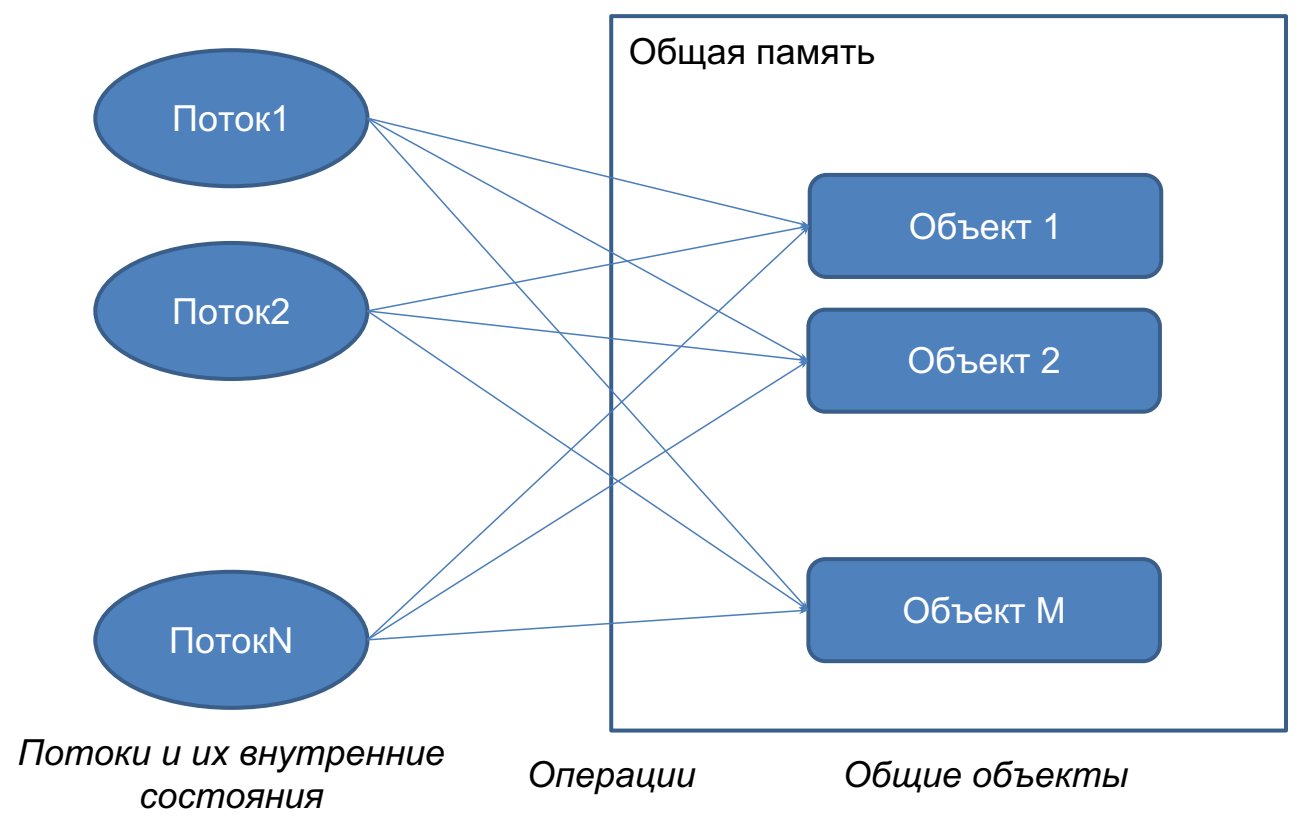
\includegraphics[width=0.7\linewidth]{pictures/CommonMemory}
	\caption{Модель с общими объектами (общей памятью)}
	\label{fig:commonmemory}
\end{figure}

\subsubsection{Общие объекты}
\begin{itemize}
	\item Потоки выполняют операции над общими, разделемыми объектами
	\item В этой моделе не важны операции внутри потоков
	\item Важна только коммуникация между потоками
	\item В этой моделе единственный тип коммуникации между потоками --- это работа с общими объектами
\end{itemize}

\subsubsection{Общие переменные}
\begin{itemize}
	\item Общие переменные --- это простейший тип общего объекта:
	\begin{itemize}
		\item У него есть значение определенного типа
		\item Есть операция чтения (read) и записи (write)
	\end{itemize}
    \item Общие переменные --- это базовые строительные блоки для многопоточных алгоритмов
    \item Модель с общими переменными --- это хорошая абстракция современных многопроцессорных систем и многопоточных ОС
    \begin{itemize}
    	\item На практике, это область памяти процесса, которая одновременно доступна для чтения и записи всем потокам этого процесса
    \end{itemize}
\end{itemize}

В теоретических трудах общие переменные называют регистрами

\subsubsection{Свойства многопоточных программ}
\begin{itemize}
	\item Последовательные программы детерминированы
	\begin{itemize}
		\item Если нет использования случайных чисел и другого явного общения с недетеминированным миром
		\item Их свойства можно установить анализируя последовательное исполнение при данных входных параметрах
	\end{itemize}
    \item Многопоточные программы в общем случае недетерминированы
    \begin{itemize}
    	\item Даже если код каждого потока детерминирован
    	\item Результат работы зависит от фактичекого исполнения при данных входных параметрах
    	\item А этих исполнений может быть много
    \end{itemize}
    \item Говорим <<Программа A имеет свойство P>> если она имеет это свойство при любом исполнении
\end{itemize}

\subsubsection{Моделирование многопотчного исполнения}

\begin{center}
	\begin{lstlisting}
	shared int x = 0, y = 0
	\end{lstlisting}
\end{center}
	
	\begin{minipage}{0.4\textwidth}
		Thread P:
		
		\begin{lstlisting}
		x = 1
		r1 = y
		stop
		\end{lstlisting}
	\end{minipage}
	\hfill
	\begin{minipage}{0.4\textwidth}
		Thread Q:
		
		\begin{lstlisting}
		y = 1
		r2 = x
		stop
		\end{lstlisting}
	\end{minipage}

\paragraph{Моделирование исполнений через чередование операций}

\begin{figure}[h!]
	\centering
	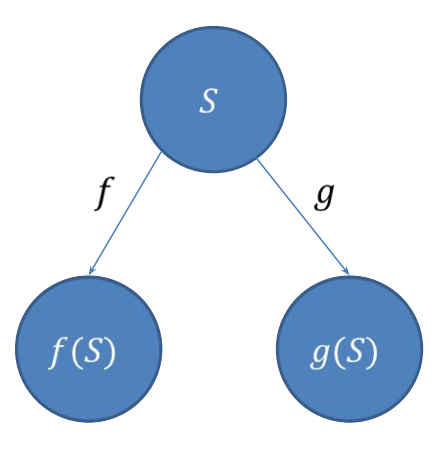
\includegraphics[width=0.3\linewidth]{pictures/Model}
	\caption{}
	\label{fig:model}
\end{figure}

\begin{itemize}
	\item $S$ --- это общее состояние:
	\begin{itemize}
		\item Состояние всех потоков (IP+locals)
		\item И состояние всех общих объектов
	\end{itemize}
    \item $f$ и $g$ --- это операции
    \begin{itemize}
    	\item Количество различных операций в каждом состоянии равно количеству потоков
    \end{itemize}
    \item $f(S)$ --- это новое состояние после применения операции $f$ к состоянию $S$ 
\end{itemize}

\begin{figure}[h!]
	\centering
	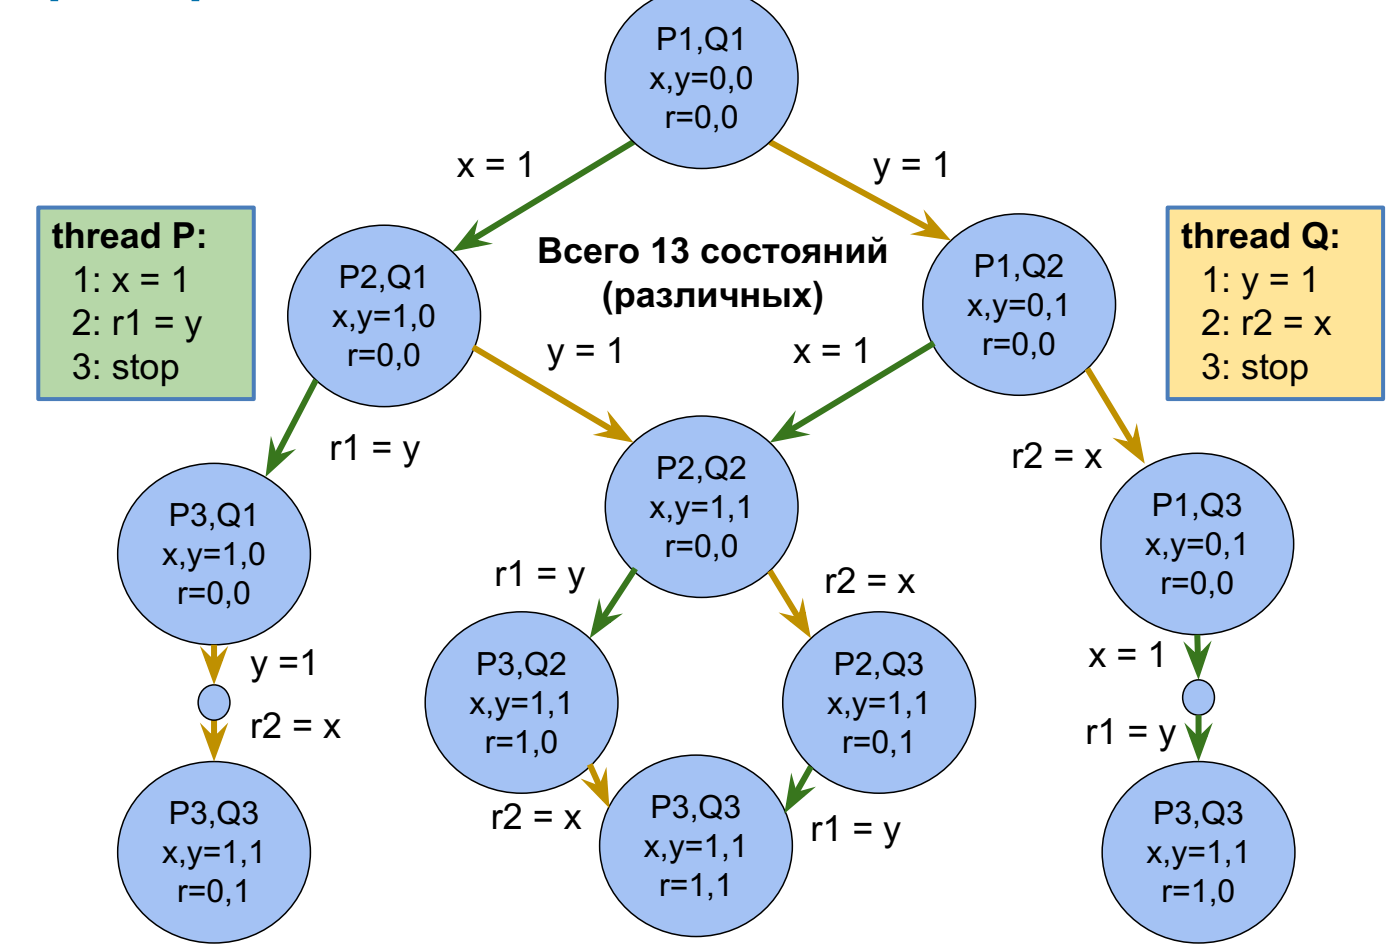
\includegraphics[width=0.5\linewidth]{pictures/Model1}
	\caption{}
	\label{fig:model1}
\end{figure}


После исполнеия этого кода для r1, r2 возможны следующие пары значений: (0, 0), (0, 1), (1, 0), (1, 1). Хотя при моделировании через чередование (рисунок~\ref{fig:model1}) первого варианта не получается. Это случается, так как в современном процессоре запись не попадает сразу в общую память, а в начале буферизируется (т.к. запись долгая операция). Поэтому мы можем прочитать старое значение, т.к. чтение быстрая операция и новые значения еще лежат в буфере. Процессор может переставить инструкции, т.к. это может ускорить однопоточный код (процессро не знает о параллельности).

\begin{figure}[h!]
	\centering
	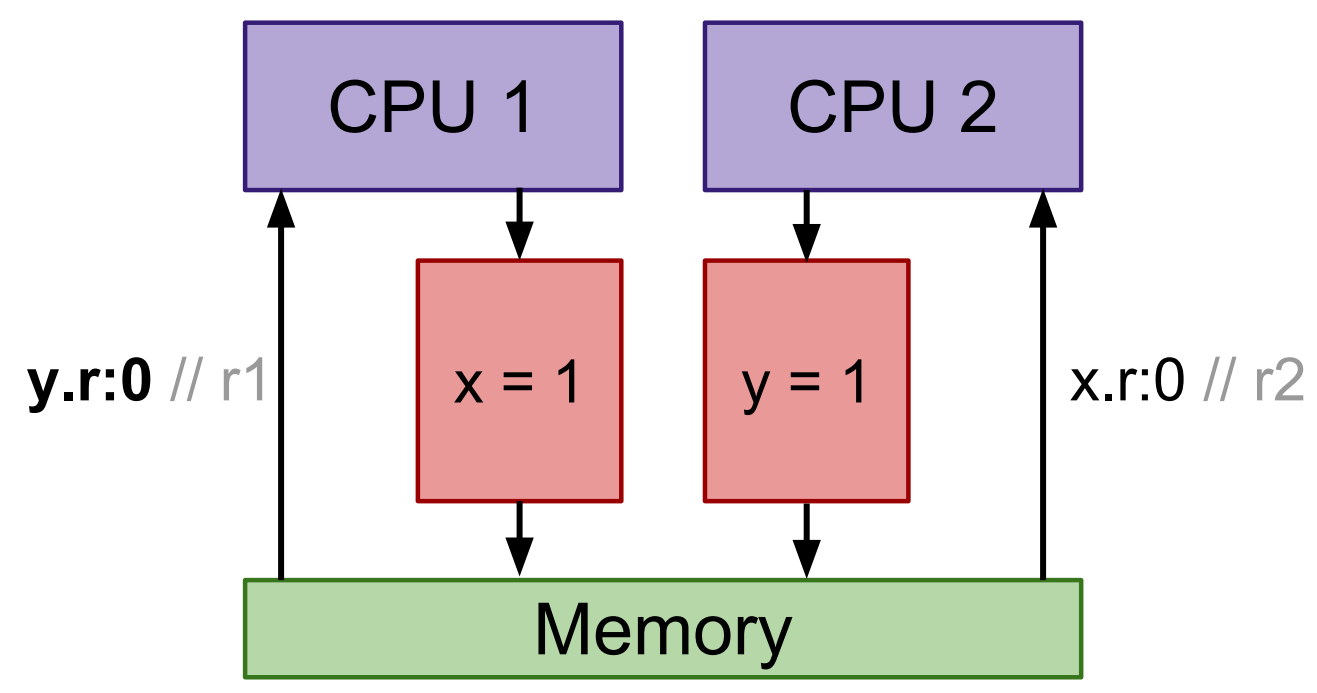
\includegraphics[width=0.4\linewidth]{pictures/Memory}
	\caption{}
	\label{fig:memory}
\end{figure}

Модель чередования не параллельна

На самом деле в настоящих процессорах операции чтения и записи не мгновенные. Они происходят паралелльно как в разных ядрах, так и в одном.

И вообще процессор обменивается с памятью сообщениями о чтении / записи и таких сообщений одновременно в обработке может быть очень много.

\section{Lock-free Treiber Stack and Michael-Scott Queue}

\section{Определения и формализм}
\subsection{Физическая реальность}
\begin{itemize}
	\item Свет (электромагнитные волны) в вакууме распространется со скоростью $\sim3\cdot10^8$ м/с.
	\begin{itemize}
		\item Это максимальный физический предел скорости
		\item За один такт процессора с частотой 3 ГГц ($3\cdot10^9$ Гц) свет в вакууме проходит всего 10 см.
	\end{itemize}
    \item Соседние процессоры физически не могут синхронизировать свою работу и физически не могут определить порядок происходящих в них событиях.
    \begin{itemize}
    	\item Они работают действительно физически параллельно
    \end{itemize}
    \item Пусть $a, b, c\in E$ --- это физически атомарные (неделимые) события, происходящие в пространстве--времени (рисунок~\ref{fig:model2})
    \begin{itemize}
    	\item Говорим <<$a$ предшествует $b$>> или <<$a$ произошло до $b$>> (и записываем $a\to b$), если свет от точки пространства--времени $a$ успевает дойти до точки пространства--времени $b$.
    	\item Это отношение частичного пордка на событиях
    \end{itemize}
\end{itemize}

\begin{figure}[h!]
	\centering
	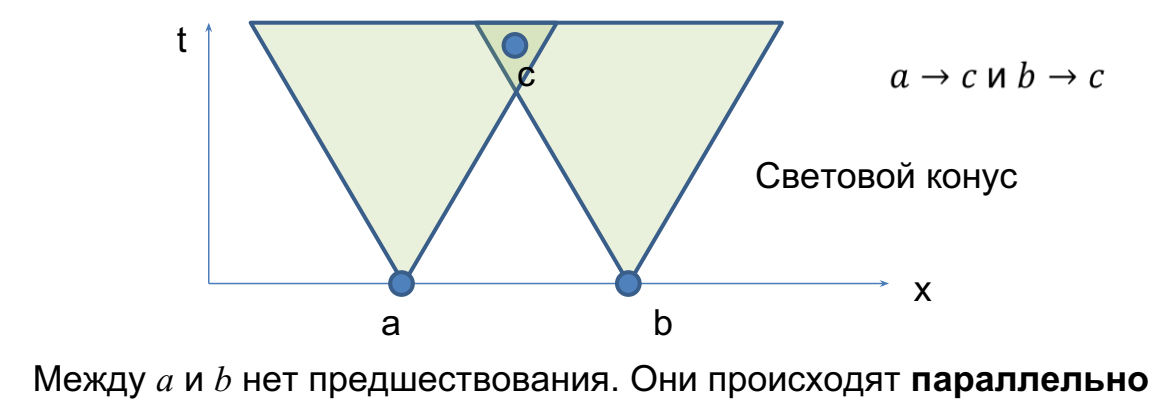
\includegraphics[width=0.5\linewidth]{pictures/Model2}
	\caption{}
	\label{fig:model2}
\end{figure}

\subsection{Модель <<произошло до>> (happens before)}
\begin{itemize}
	\item Впервые введена Л.~Лампортом в 1978 году.
	\item Исполнение системы --- это пара ($H, \to_H$)
	\begin{itemize}
		\item $H$ --- это множество операций $e, f, g, \ldots$ (чтение и запись ячеек памяти и т.~п.) произошедших во время исполнения
		\item $\to_H$ --- это транзитивное, антирефлексивное, ассимметричное отношение (частичный строгий порядок) на множестве операций
		\item $e\to_Hf$ означает, что <<$e$ произошло до $f$ в исполнении $H$>>. Чаще всего исполнение $H$ понятно из контекста и опускается 
	\end{itemize}
    \item Две операции $e$ и $f$ параллельны ($e\parallel f$), если $e\nrightarrow f\wedge f\nrightarrow e$.
    \item Система --- это набор всех возможных исполнений системы
    \item Говорим, что <<система имеет свойство P>>, если каждое исполнение системы имеет свойство P.
\end{itemize}

\subsection{Модель глобального времени}

В этой моделе каждая операция --- это временный интервал (рисунок~\ref{fig:model3}) $e=[t_{inv}(e), t_{res}(e)]$ где $t_{inv}(e), t_{res}(e)\in\mathbb{R}$ и
$$
e\to f\stackrel{\mathrm{def}}{=}t_{res}(e)<t_{inv}(f)
$$

\begin{figure}
	\centering
	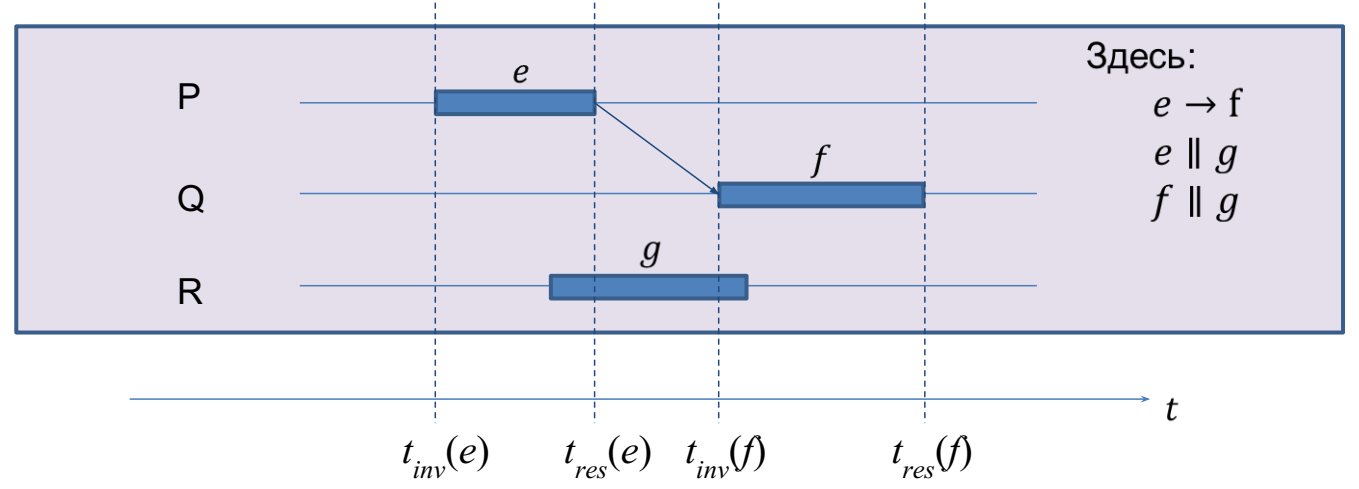
\includegraphics[width=0.5\linewidth]{pictures/Model3}
	\caption{Модель глобального времени}
	\label{fig:model3}
\end{figure}

\subsection{Обсуждение глобального времени}
На самом деле никакого глобального времени нет и не может быть из--за физических ограничений.

\begin{itemize}
	\item Это всего лишь механизм, позволяющий визуализировать факт существования параллельных операций.
	\item При доказательстве различных фактов и анализе свойств [исполнений] системы время не используется
	\begin{itemize}
		\item Анализируютя только операции и отношения <<произошло до>>
	\end{itemize}
\end{itemize}

\subsection{<<Произошло до>> на практике}
\begin{itemize}
	\item Современные языки программирования предоставляют программисту операции синхронизации:
	\begin{itemize}
		\item Специальные механизмы чтения и записи переменных
		\item Создание потоков и ожидание их завершения
		\item Различные другие библиотечные примитивы для синхронизации
	\end{itemize}
    \item Модель памяти языка программирования определяет то, каким образом исполнение операций синхронизации создает отношение <<произошло до>>
    \begin{itemize}
    	\item Без них разные потоки выполняются параллельно
    	\item Можно доказать те или иные свойства многопоточного кода, используя гарантии на возможные исполнения, которые дает модель памяти
    \end{itemize}
\end{itemize}

\subsection{Свойства исполнений над общими объектами}
\subsubsection{Операции над общими объектами}
\begin{figure}[h!]
	\centering
	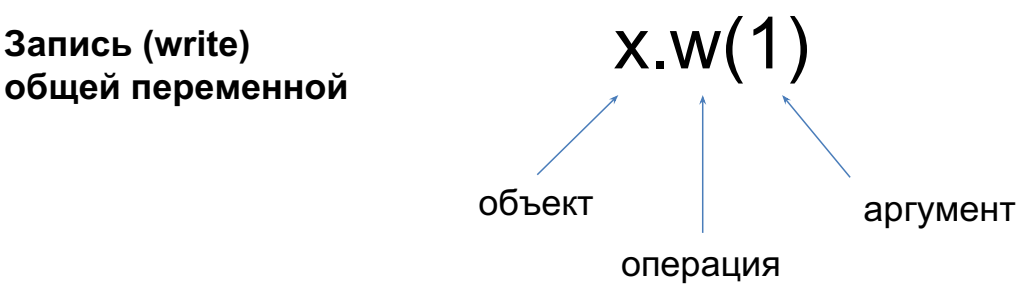
\includegraphics[width=0.6\linewidth]{pictures/Write}
	\caption{Запись}
	\label{fig:write}
\end{figure}

\begin{figure}[h!]
	\centering
	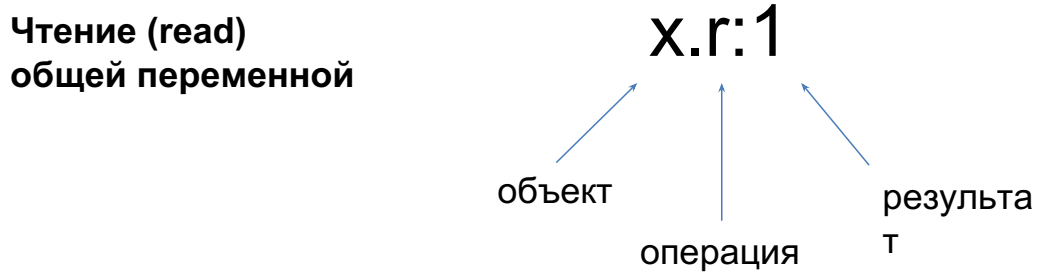
\includegraphics[width=0.6\linewidth]{pictures/Read}
	\caption{Чтение}
	\label{fig:read}
\end{figure}


\subsubsection{Последовательное исполнение}
\begin{defenition}
	Исполнение системы называется последовательным, если все операции линейно--упорядочены отношением <<произошло до>>, то есть $\forall e, f\in H\colon (e=f)\vee(e\to f)\vee(f\to e)$.
\end{defenition}

\begin{figure}
	\centering
	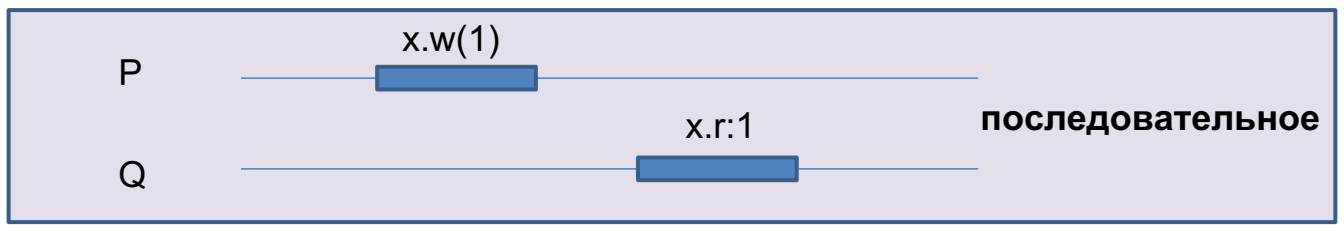
\includegraphics[width=0.4\linewidth]{pictures/Model4}
	\caption{Последовательное исполнение}
	\label{fig:model4}
\end{figure}

\begin{figure}
	\centering
	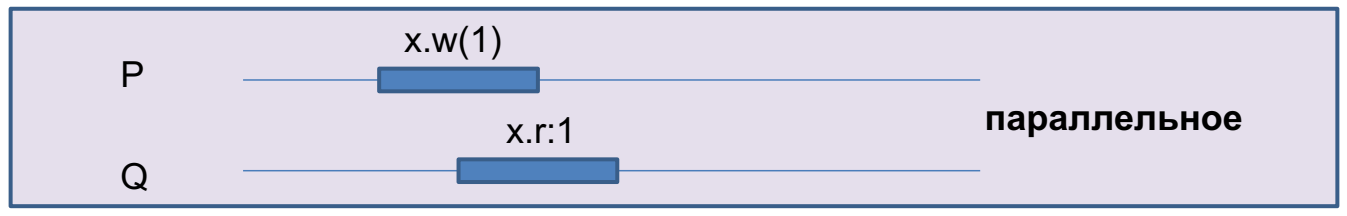
\includegraphics[width=0.4\linewidth]{pictures/Model5}
	\caption{Параллельное исполнение}
	\label{fig:model5}
\end{figure}

\subsubsection{Конфликты и гонки данных (data race)}
\begin{itemize}
	\item \begin{defenition}
		Две операции над одной переменной, одна из которых запись, называются конфликтующими.
	\end{defenition}
    Конфликтующие операции не коммутируют в модели чередования.
	\item \begin{defenition}
		Если две конфликтующие операции произошли параллельно, то такая ситуация называется гонка данных (data race).
	\end{defenition} 
	\begin{itemize}
		\item Это свойство конкретного исполнения.
	\end{itemize}
\end{itemize}

\begin{defenition}
	Программа, в любом допустимом исполнении которой (с точки зрения модели памяти) нет гонок данных, называется корректно синхронизированной.
\end{defenition}

\subsubsection{Правильное исполнение} 
\begin{itemize}
	\item $H|_p$ --- сужение исполнения на поток $P$, то есть исполнение, где остались только операции, происходящие в потоке $P$.
	\item \begin{defenition}
		Исполнение называется {\bfseries правильным (well-formed)}, если его сужение на каждый поток $P$ является последовательным (рисунок~\ref{fig:model6}).
	\end{defenition} 
\end{itemize}
\begin{figure}
	\centering
	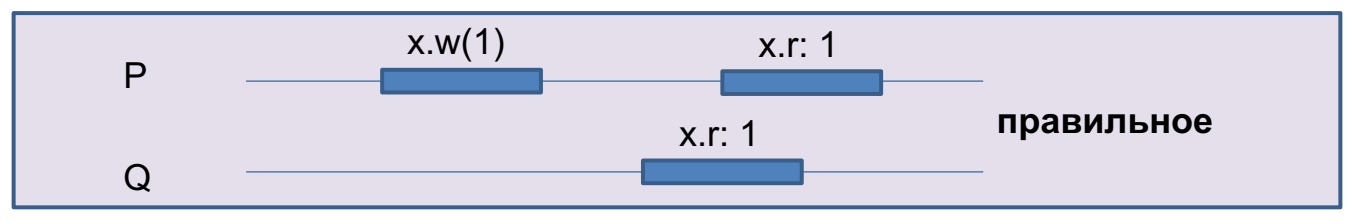
\includegraphics[width=0.5\linewidth]{pictures/Model6}
	\caption{Правильное исполнение}
	\label{fig:model6}
\end{figure}

\subsubsection{Правильное исполнение и нотация}
\begin{itemize}
	\item $H|_p$ --- сужение исполнения на поток $P$ --- это множестов всех операций $e\in H$, таких что $proc(e)=P$.
	\begin{itemize}
		\item Исполнение называется {\bfseries правильным (well-formed)}, если его сужение на каждый поток $P$ является последовательным.
		\item Задается программой, которую выполняет поток.
		\item \begin{defenition}
			Объединение всех сужений на потоки называют {\bfseries пргораммным порядком} (po = program order).
		\end{defenition}
	    \item Нас интерисуют только правильные исполнения.
	\end{itemize}
    \item $H|_x$ --- сужение истории на объект $x$ --- это множество операций $e\in H$, таких что $obj(e)=x$. В правильном исполнении сужение на объект е обязательно является последовательным.
\end{itemize}

\subsubsection{Последовательная спецификация объекта}
Если сужение исполнения на объект $H|_x$ является последовательным, то можно проверить его на соответсвие {\bfseries последовательной спецификации объекта}.

\subsubsection{Допустимое последовательное исполнение}
\begin{defenition}
	Последовательное исполнение является {\bfseries допустимым (legal)}, если выполнены последовательные спецификации всех объектов (рисунок~\ref{fig:model7}).
\end{defenition}

\begin{figure}[h!]
	\centering
	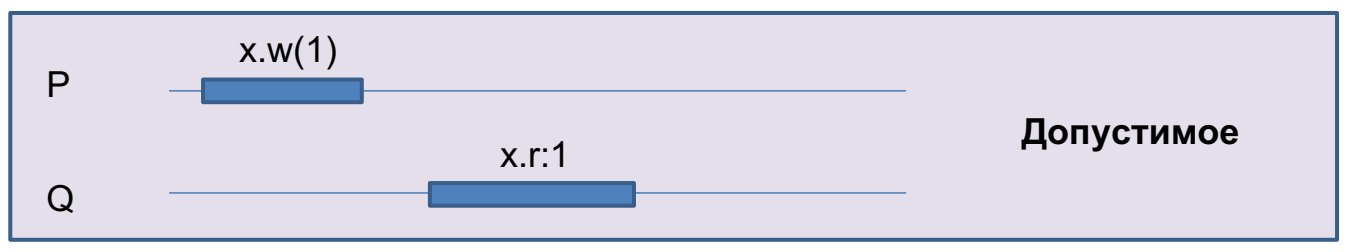
\includegraphics[width=0.5\linewidth]{pictures/Model7}
	\caption{Допустимое исполнение}
	\label{fig:model7}
\end{figure}

\begin{figure}[h!]
	\centering
	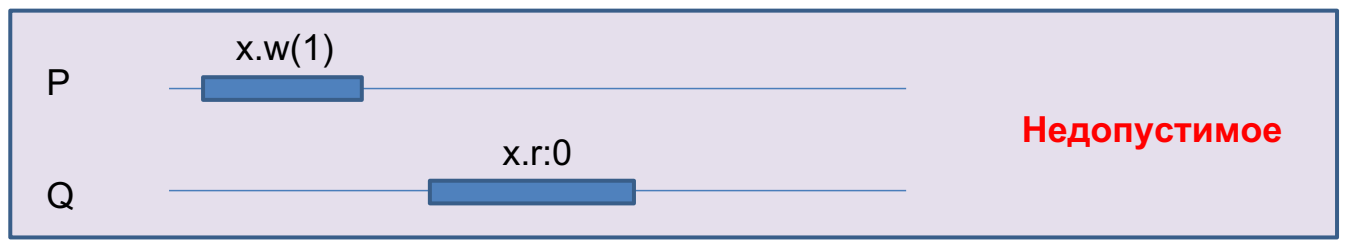
\includegraphics[width=0.5\linewidth]{pictures/Model8}
	\caption{Недопустимое исполнение}
	\label{fig:model8}
\end{figure}

\subsubsection{Условия согласованности (корректности)}
{\bfseries Корректные} последовательные программы должны считаться {\bfseries согласованными}.

Условия согласованности:
\begin{itemize}
	\item Согласованность при покое
	\item Последовательная согласованность
	\item Лианеризуемость
	\item и другие
\end{itemize}

\paragraph{Последовательная согласованность}
\begin{defenition}
	Исполнение {\bfseries последовательно согласованно}, если ему можно сопоставить эквивалентное ему допустимое исполнение, сохраняющее его программный порядок (рисунок~\ref{fig:model9}).
\end{defenition}

\begin{figure}[h!]
	\centering
	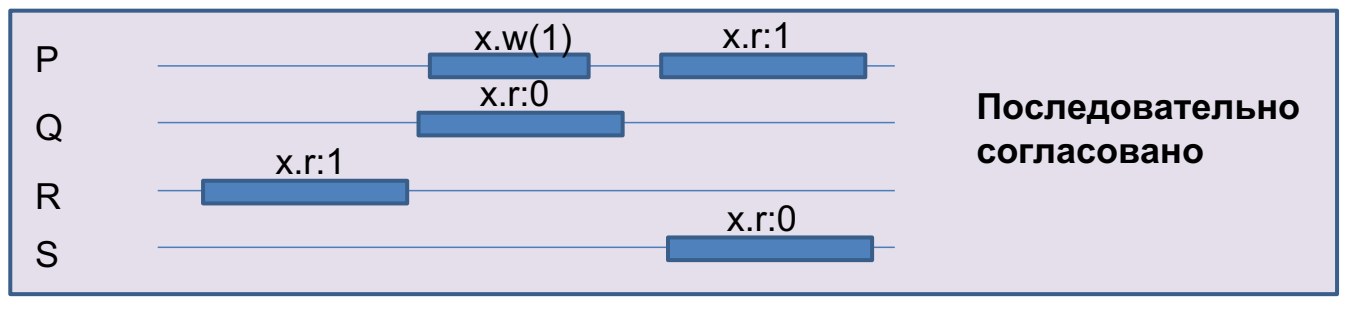
\includegraphics[width=0.5\linewidth]{pictures/Model9}
	\caption{Последовательно согласованно}
	\label{fig:model9}
\end{figure}

Последовательная согласованность на каждом объекте исполнения не влечет последовательную согласованость всего исполнения (рисунок~\ref{fig:model10})

\begin{figure}[h!]
	\centering
	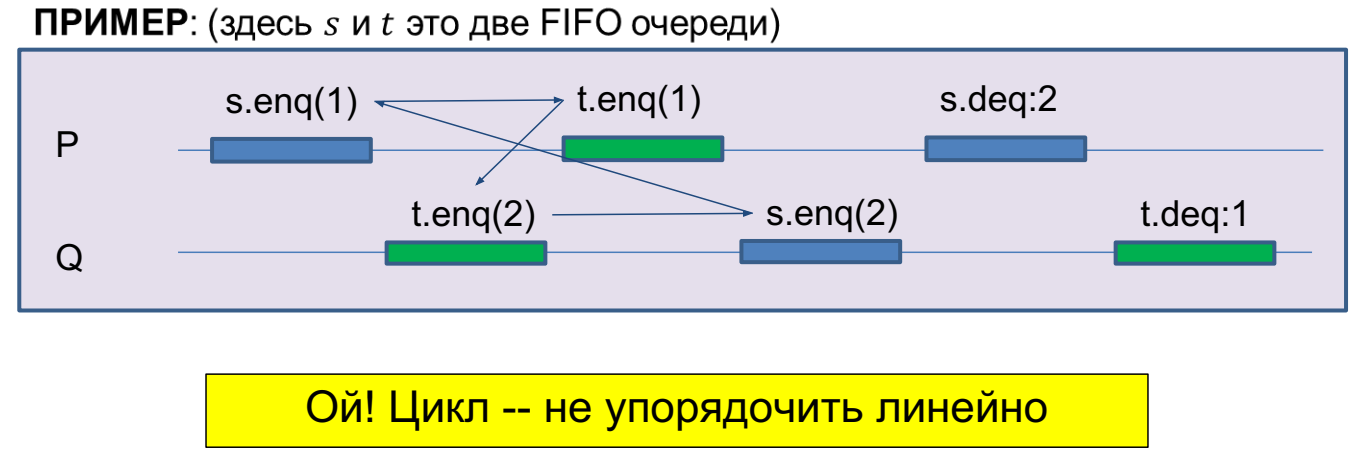
\includegraphics[width=0.7\linewidth]{pictures/Model10}
	\caption{}
	\label{fig:model10}
\end{figure}

Модель памяти языков программрования и системы исполнения кода используют последовательную согласованность для своих формулировок.

\paragraph{Лианеризуемость}
\begin{defenition}
	Исполнение {\bfseries лианеризуемо}, если можно сопоставить эквивалентное ему допустимое последовательное исполнение, которое сохраняет отношение <<произошло до>>. 
\end{defenition}

Свойства лианеризуемости:
\begin{itemize}
	\item В лианеризуемом исполнении каждой операции $e$ можно сопоставить точку глобального времени ({\bfseries точку лианеризации}) $t(e)\in\mathbb{R}$ так, что время различных операций различно и
	$$
	e\to f\Rightarrow t(e)<t(f)
	$$
	\item Лианеризуемость {\bfseries локальна}. Лианеризуемость исполнения на каждом объекте эквивалентна лианеризуемости системы целиком.
	\item \begin{defenition}
		Операции над лианеризуемыми объектами называют {\bfseries атомарными}.
	\end{defenition}
\end{itemize}

\paragraph{Лианеризуемость в глобальном времени}

В глобальном времени исполнение лианеризуемо тогда и только тогда, когда точки лианеризуемости можно выбрать так, что
$$
\forall e\colon t_{inv}(e)<t(e)<t_{res}(e)
$$

\begin{figure}[h!]
	\centering
	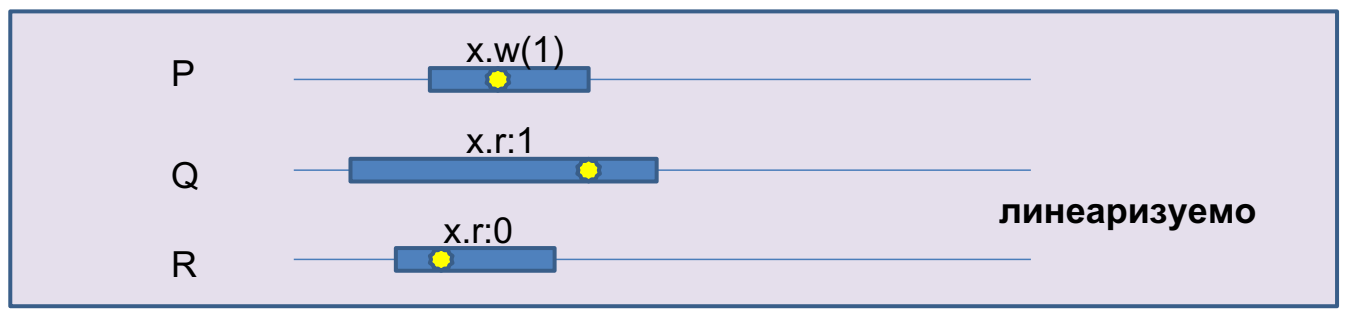
\includegraphics[width=0.5\linewidth]{pictures/Model11}
	\caption{Лианеризуемость}
	\label{fig:model11}
\end{figure}

\subsection{Лианеризуемость}
Исполнение системы, выполняющей операции над лианеризуемыми объектами, можно анализировать в модели чередования.

Из более простых лианеризуемых объектов можно сделать лианеризуемые объекты более высокого уровня. 

Когда говорят, что объект безопасен для использования из нескольких потоков, подразумевают, что операции над ним лианеризуемы.

\subsubsection{Применительо к Java}
\begin{itemize}
	\item Все операции над volatile полями в Java, согласно JMM, являются операциями синхронизации, которые всегда линейно--упорядочены в любом исполнении и соглосованы с точки зрения чтения/записи.
	\item Но операции над не volatile полями могут нарушать не только лианеризуемость, но даже последовательную согласованность, при отсутствии синхронизации.
	\item Если программа корректно синхронизированна, то JMM дает гарантию последовательно согласованного исполнения всего кода. 
\end{itemize}

\section{Построение атомарных объектов и блокировки}
\subsection{Сложные и составные операции}
\subsubsection{Формализация сложных операций}
\begin{itemize}
	\item Операция $e\in H$ может быть сложной. Даже чтение из памяти это продолжительное по времени действие, много шагов.
	\item {\bfseries Событие}
	\begin{itemize}
		\item Неделимое, простое физическое действие
		\item Множество событий обозначим $G$
		\item Каждая операция это множество событий $e\subset G$
	\end{itemize}
    \item Из всех событий выделяют два наиболее важных
    \begin{itemize}
    	\item Вызов операции $inv(e)\in G$
    	\item Завершение операции $res(e)\in G$
    \end{itemize}
    \item Декомпозиция исполнения --- ($H$, $G$, $\to_G$, inv, res)
    \begin{itemize}
    	\item $H$ --- это множество операций ($\forall e\in H\colon e\subset G$)
    	\item $G$ --- это множество событий
    	\item $\to_G$ --- отношение <<произошло до>> на событиях из $G$.
    	\item inv, res --- фукции из $H$ в $G$, такие что:
    	$$
    	\forall e\in H\colon inv(e)\to_Gres(e)
    	$$
    	$$
    	\forall e\in H, g\in e, g\ne inv(e), g\ne res(e)\colon inv(e)\to_Gg\to_Gres(e)
    	$$
    \end{itemize}
\end{itemize}

\section{Consensus}
\subsection{Задача о консенсусе}

Каждый поток использует объект Consensus один раз

\begin{itemize}
	\item Согласованность: все потоки должны вернуть одно и тоже значение из метода decide
	\item Обоснованность: возвращенное значение было входным значением какого-то из потоков
	\item Без ожидания
\end{itemize}

\subsection{Консенсусное число}
\begin{itemize}
	\item Если с помощью класса атомарных объектов C и атомарных регистров можно реализовать консенсусный протокол без ожидания с помощью детерминированного алгоритма для N потоков (и не больше), то говорят, что у класса C консенсусное число N.
	\item \begin{theorem}
		Атомарные регистры имеют консенсусное число 1.
	\end{theorem} 
\end{itemize}

\subsection{Модель}
\begin{itemize}
	\item x--валентное состояние системы --- консенсус во всех нижестоящих листьях будет x.
	\item Бивалентное состояние --- возможен консенсус как 0, так и 1.
	\item Критическое состояние --- такое бивалентное состояние, у которого все дети одновалентны
\end{itemize}

\subsection{Read--Modify--Write регистры}

\subsection{Универсальность консенсуса}
\begin{theorem}
	Любой последовательный объект можно реализовать без ожидания для N потоков, используя консенсусный проткол для N потоков
\end{theorem}

\section{Алгоритмы без блокировок: Построение на регистрах}
\subsection{Безусловные условия прогресса}
\begin{itemize}
	\item Отсутствие помех --- Если несколько потоков пытаются выполнить операцию, то любой из них должен выполнить ее за конечное время, если все другие остановить в любом месте
	\item Отсутствие блокировки --- если несколько потоков пытаются выполнить операцию, то хотя бы один из них должен выполнить ее за конечное время, независимо от действия или бездействия других потоков
	\item Отсутствие ожидания --- если поток хочет выполнить операцию, то он выполнит ее за конечное время независимо от других потоков
\end{itemize}

\section{Практические построения на списках}

\subsection{МНожество на односвязном списке}

\begin{lstlisting}
interface Set{
   fun add(key: Int)
   fun contains(key: Int): Boolean
   fun remove(key: Int)
}
\end{lstlisting}

Элементы упорядочены по возрастанию (рисунок~\ref{fig:set1}).

\begin{figure}
	\centering
	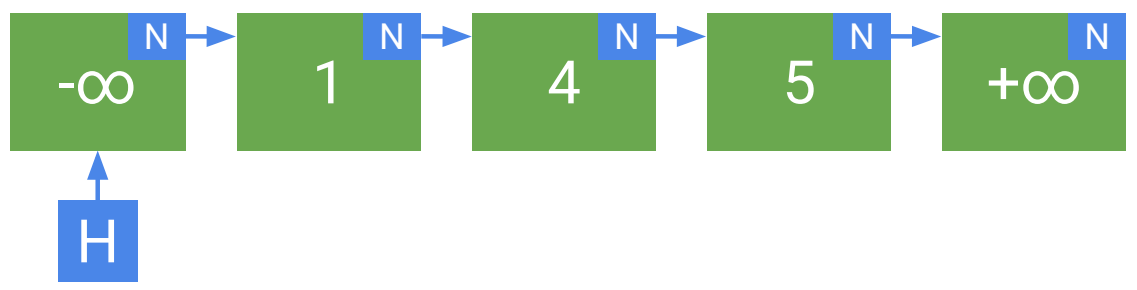
\includegraphics[width=0.4\linewidth]{pictures/Set1}
	\caption{Односвязный список}
	\label{fig:set1}
\end{figure}

Пустой список состоит из двух граничных элементов (рисунок~\ref{fig:set2}).

\begin{figure}
	\centering
	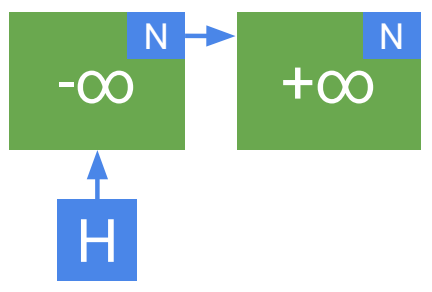
\includegraphics[width=0.4\linewidth]{pictures/Set2}
	\caption{Пустой список}
	\label{fig:set2}
\end{figure}

\subsubsection{Алгоритм}

\begin{itemize}
	\item Элементы упорядочены по возрастанию
	\item Ищем окно $(cur, next)$, что $cur.KEY<key\leqslant next.KEY$ и $cur.N=next$
	\item Искомый элемент будет в $next$
	\item Новый элемент добавляем между $cur$ и $next$
\end{itemize}

\subsubsection{Псевдокод}

\lstinputlisting{SetEasy.kt}

\subsubsection{Проблема}

При параллельном удалении соседних элементов могут возникнуть проблемы с перенаправление ссылок: например, мы успели удалить $cur$ перед тем как переназначить ссылки и у нас взникнет NullPointerException или список просто разорвется

\subsection{Грубая синхронизация}

\begin{itemize}
	\item Coarse-grained locking
	\item Используем общую блокировку для всех операций
	\item $\Rightarrow$ обеспечиваем последовательное исполнение
	\item В Java для этого можно использовать synchronized и java.utils.concurrent.locks.ReentrantLock
\end{itemize}

\subsection{Тонкая блокировка}

\begin{itemize}
	\item Fine-Grained locking
	\item Своя блокировка на каждый элемент
	\item При поиске окна держим блокировку на текущий и следующий элемент
\end{itemize}

\subsubsection{Корректность}

\begin{itemize}
	\item Поиск окна: запись и чтение $cur.N$ не может происходить параллельно
	\item Модификация: во время изменения окно защищено блокировкой $\Rightarrow$ атомарно
	\item $\forall k$: операции с ключем $k$ лианеризуемы $\Rightarrow$ всё исполнение лианеризуемо
	\item Операции с ключем $k$ упорядочены взятием блокировки
\end{itemize}

\subsection{Оптимистичная синхронизация}

\subsubsection{Алгоритм абстрактной операции}

\begin{enumerate}
	\item Найти окно $(cur, next)$ без синхронизации
	\item Взять блокировки на $cur$ и $next$
	\item Проверит инвариант $cur.N=next$
	\item Проверить, что $cur$ не удалён
	\item Выполнить операцию
	\item При любой ошибке начать занаво
\end{enumerate}

\subsubsection{Проверка, что узел не удалён}

\begin{itemize}
	\item Держи блокировку на $cur$ и $cur$ удалён $\Rightarrow$ не увидим при проходе
	\item Попробуем найти $cur$ ещё раз за $O(n)$ и проверим, что $cur.N=next$
\end{itemize}

\subsubsection{Валидация окна}

\begin{lstlisting}
fun validate(cur: Node, next: Node): Boolean {
    node := head
    while (node.key < cur.key) {
        node = node.N
    }    
    return (cur, next) = (node, node.N)
}
\end{lstlisting}

\subsubsection{Корректность}

\begin{itemize}
	\item Поиск: запись и чтение $cur.N$ связаны отношением <<произошло до>>
	\item Можем говорить о лианеризуемости операция над одинаковыми ключами
	\item Точка лианеризации - взятие блокировки над $cur$
\end{itemize}

\subsection{Ленивая синхронизация}

\subsubsection{Идея ленивого удаления}

\begin{itemize}
	\item Добавим в Node поле removed типа Boolean
	\item Удаление в две фазы
	      \begin{enumerate}
	      	\item $node.removed=true$ --- логическое удаление
	      	\item Физическое удаление из списка
	      \end{enumerate}
    \item Инвариант: все не удалённые вершины в списке
    \item $\Rightarrow$ теперь не над проходить по всему списку в validate()
\end{itemize}

\subsubsection{Псевдокод}

\begin{lstlisting}
fun validate(cur: Node, next: Node): Boolean {
    return !cur.removed && !next.removed && cur.N=next
}
\end{lstlisting}

\subsection{Неблокирующая синхронизация}

\subsubsection{Неблокирующий поиск}

\begin{itemize}
	\item На момент чтения поля $N$ видим состояние на момент записи $N$ или новее
	\item $\Rightarrow$ можем не брать блокиовку при поиске
\end{itemize}

\begin{lstlisting}
fun contains(key: Int): Boolean {
    (cur, next) := findWindow(key)
    return next.key = key
}
\end{lstlisting}

\subsubsection{Неблокирующая модификация}

\begin{itemize}
	\item Объединим N и removed в одну переменную, пару $(N, removed)$
	\item Будем менять $(N, removed)$ атомарно
	\item Каждая операция модификации будет выполняться одни успешным CAS-ом
	\item В Java для этого есть AtomicMarkableReference
\end{itemize}

\section{Lock-free хеш таблица с открытой адресацией}

\subsection{ConcurrentHashMap}

\begin{itemize}
	\item Работает за $O(1)$ в среднем
	\item Использует внутри блокировки $\Rightarrow$ не так хорошо масштабируется
	\item Хранит списки при коллизии (рисунок~\ref{fig:concurrenthashmap1})
	\begin{itemize}
		\item $\Rightarrow$ лишние cache miss-ы
		\item зато может хранить дерево при постоянных коллизиях (рисунок~\ref{fig:concurrenthashmap2})
	\end{itemize}
\end{itemize}

\begin{figure}[h!]
	\centering
	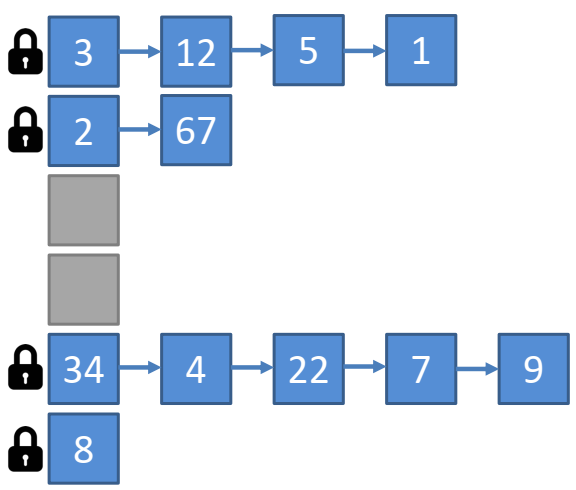
\includegraphics[width=0.4\linewidth]{pictures/ConcurrentHashMap1}
	\caption{Simple ConcureentHashMap}
	\label{fig:concurrenthashmap1}
\end{figure}

\begin{figure}[h!]
	\centering
	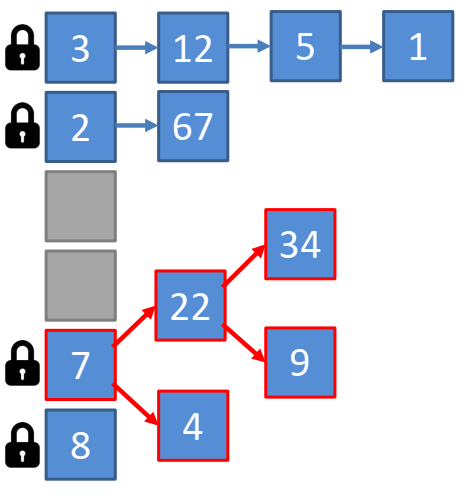
\includegraphics[width=0.4\linewidth]{pictures/ConcurrentHashMap2}
	\caption{ConcurrentHashMap with tree}
	\label{fig:concurrenthashmap2}
\end{figure}

\subsection{Skip List}

\begin{itemize}
	\item Работает за $O(\log(n))$ в среднем
	\item <<Дерево>> списков
	\begin{itemize}
		\item Много лишних объектов
		\item $\Rightarrow$ постоянные cache miss-ы и нагружает GC 
	\end{itemize}
    \item И вообще это не хеш таблица
\end{itemize}

\begin{figure}[h!]
	\centering
	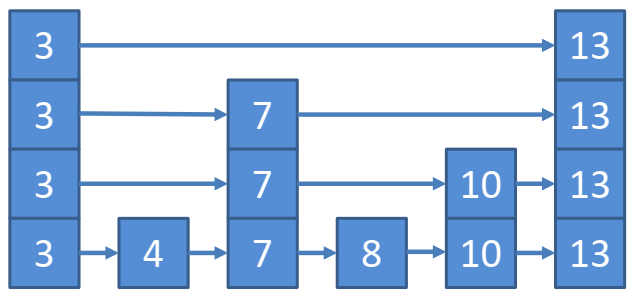
\includegraphics[width=0.4\linewidth]{pictures/SkipList}
	\caption{Skip List}
	\label{fig:skiplist}
\end{figure}

\subsection{Потенциальные проблемы}
\begin{itemize}
	\item ConcurrentHashMap
	\begin{itemize}
		\item Использует внутри блокировки $\Rightarrow$ не lock-free\footnote{Это важно для высоконагруженных систем}
		\item Использует списки $\Rightarrow$ cache miss-ы
	\end{itemize}
    \item Много <<лишних>> объектов
    \item Постоянные cache miss-ы
\end{itemize}

\subsection{NonBlockingHashMap}

\begin{itemize}
	\item Использует открытую адресацию
	\item Lock-free
	\begin{itemize}
		\item Гарантирует, что система не стоит на месте даже при неудачном scheduling-е
		\item Можно вставлять читать во время перехеширования
	\end{itemize}
\end{itemize}

\begin{lstlisting}
public T getInternal(long key) {
    int i = index(key);
    long k;
    int probes = 0;
    while ((k = keys.get(i)) != key) {
        if (k == NULL_KEY) 
            return null;
        if (++probes >= MAX_PROBES)
            return null;
        if (i == 0) 
           i = length;
        i--;
    }
    return values.get(i);
}
\end{lstlisting}

\subsubsection{Пара деталей}

\begin{itemize}
	\item Теория говорит, что размер таблицы должен быть простым числом, но так как операция взятия по модулю дорогая, то на практике используется степени двойки, для которых требуется только сдвиг
	\item В теории при поиске элемента лучше смотреть не на следующий элемент, но на практике наоборот, так как следующий уже скорее всего закэширован  
\end{itemize}

\subsection{MRSW хеш таблица (рисунок~\ref{fig:element1})}

Увеличение в случае одного писателя:
\begin{enumerate}
	\item Создаем новую таблицу
	\item Копируем элементы
	\item Меняем ссылку на таблицу
\end{enumerate}

\begin{figure}
	\centering
	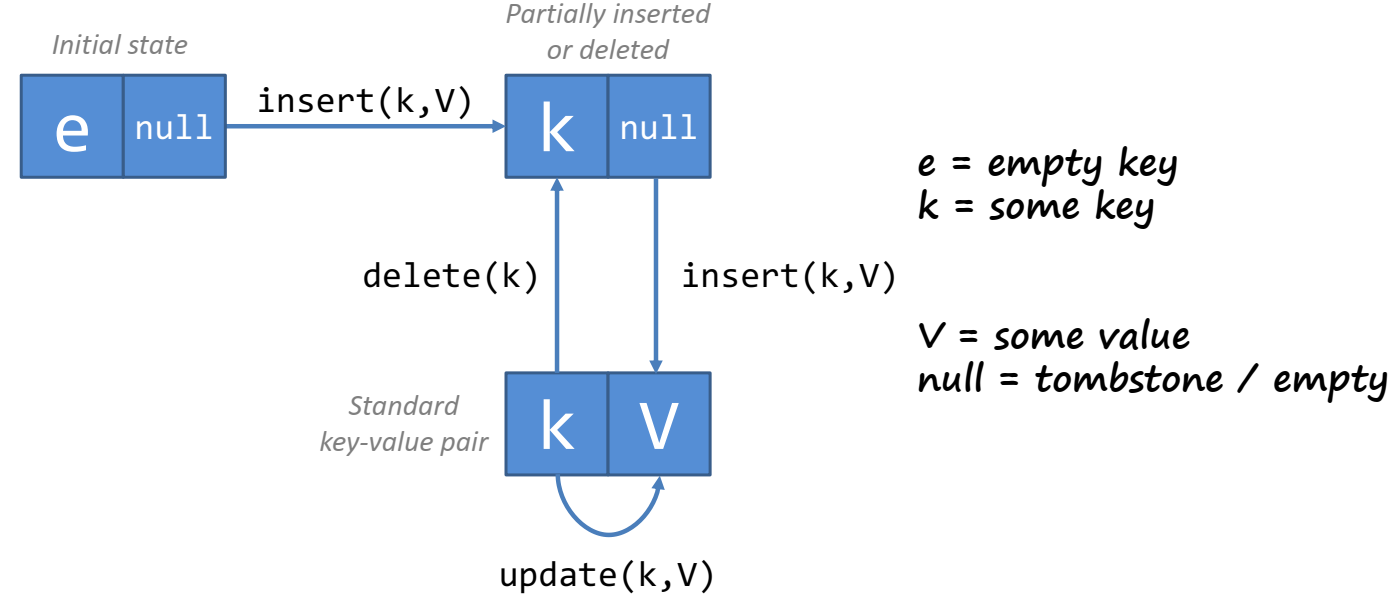
\includegraphics[width=0.4\linewidth]{pictures/Element1}
	\caption{Простая жизнь ячейки}
	\label{fig:element1}
\end{figure}

\subsection{MRMW хеш таблица}

\begin{figure}[h!]
	\centering
	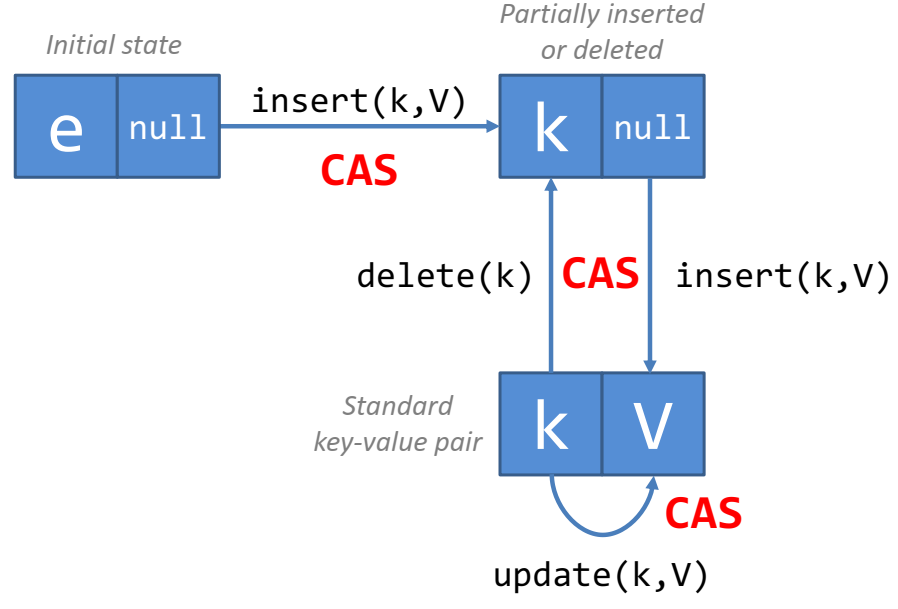
\includegraphics[width=0.4\linewidth]{pictures/Element2}
	\caption{Жизнь ячейки без переноса}
	\label{fig:element2}
\end{figure}

\begin{figure}[h!]
	\centering
	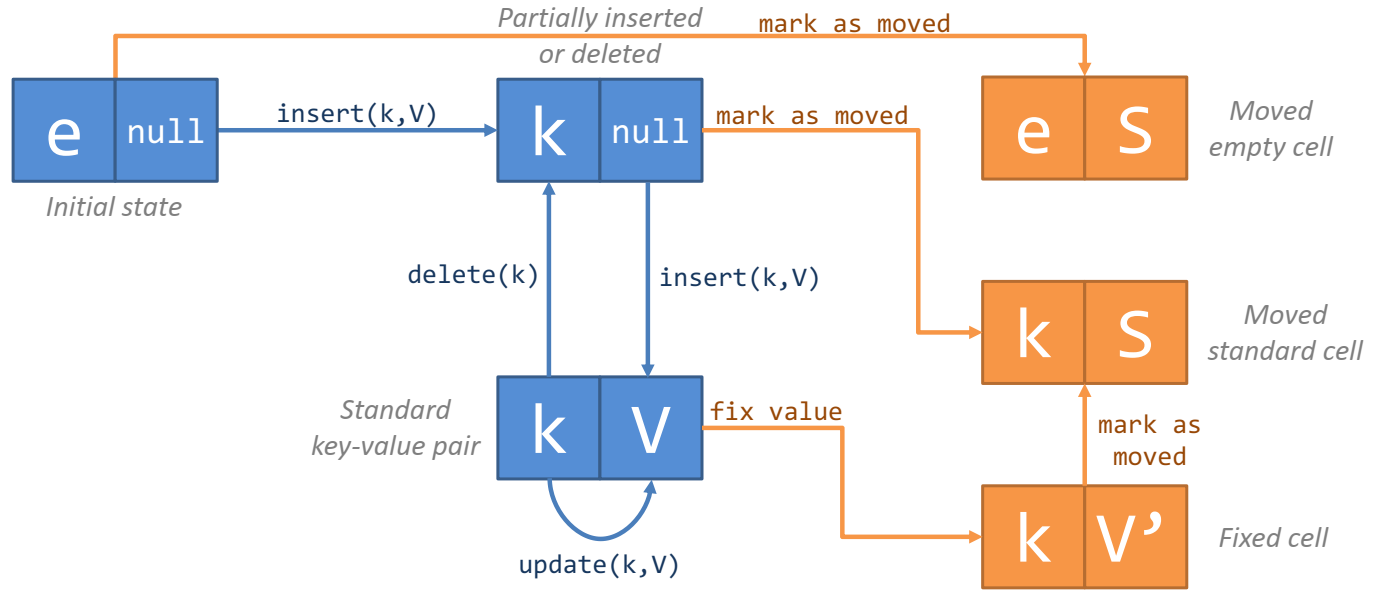
\includegraphics[width=0.4\linewidth]{pictures/Element3}
	\caption{Жизнь ячейки с переносом}
	\label{fig:element3}
\end{figure}

\begin{figure}
	\centering
	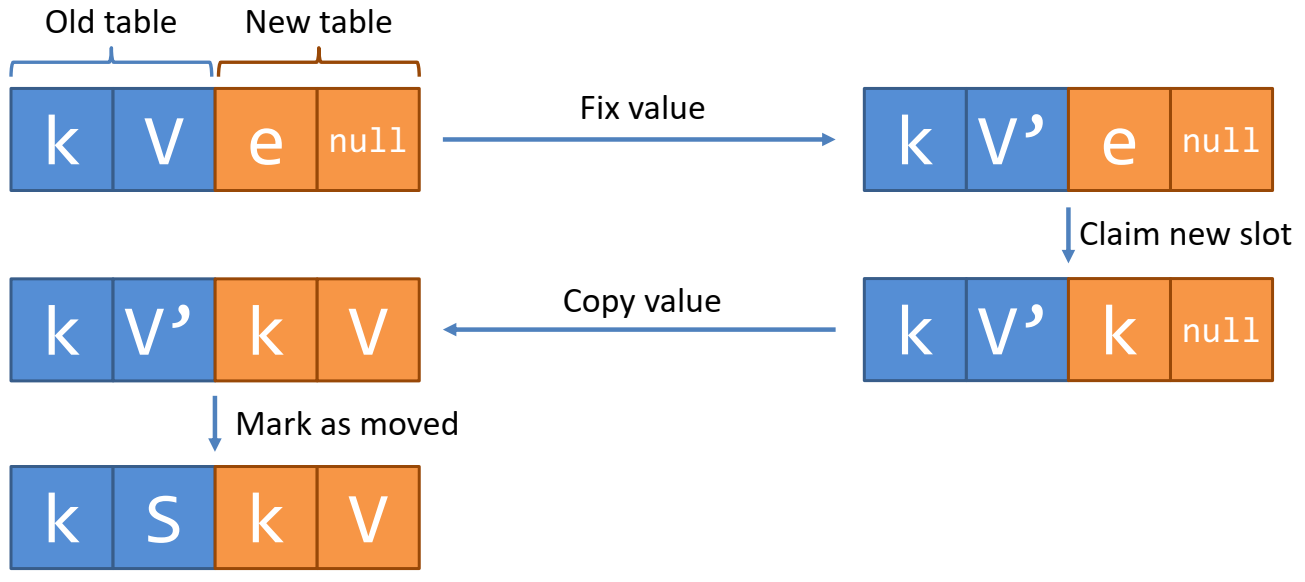
\includegraphics[width=0.4\linewidth]{pictures/Element4}
	\caption{Другой взгляд на перенос}
	\label{fig:element4}
\end{figure}

\subsubsection{Кооперация при переносе}

\begin{itemize}
	\item Переносить блоками по k элементов
	\item Переносом занимается один выделенный поток
\end{itemize}

\section{CASN}
\subsection{Списки против массивов}
\begin{itemize}
	\item Список (рисунок~\ref{fig:list})
	\begin{itemize}
		\item $3*N$ слов памяти (минимум) (рисунок~\ref{fig:list1})
		\item при многопотном использовании хватает одного CAS для добавления элемента (рисунок~\ref{fig:list2})
	\end{itemize}
    \item Массив (рисунок~\ref{fig:array})
    \begin{itemize}
    	\item $5+N$ слов памяти (до $5+2*N$ при х2 резерве) (рисунок~\ref{fig:array1})
    	\item Как минимум в два раз быстрее работает с памятью (обычно растет на попрядок) (при однопоточной работе)
    	\item Для добавления нужно CAS2 (для size и элемента) --- эта операция не поддерживается на процессорах (рисунок~\ref{fig:array2})
    \end{itemize}
\end{itemize}

\begin{figure}[h!]
	\centering
	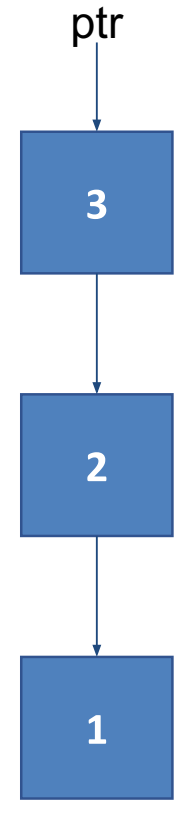
\includegraphics[width=0.05\linewidth]{pictures/List}
	\caption{Список}
	\label{fig:list}
\end{figure}

\begin{figure}[h!]
	\centering
	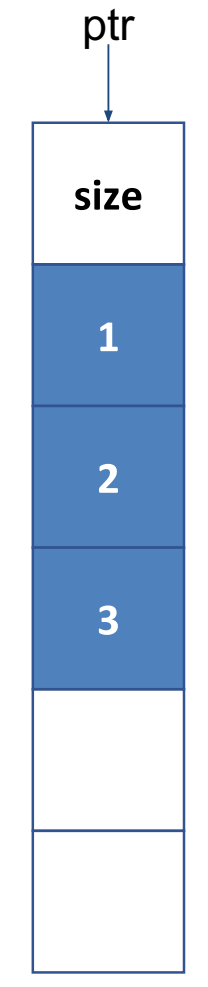
\includegraphics[width=0.05\linewidth]{pictures/Array}
	\caption{Массив}
	\label{fig:array}
\end{figure}

\begin{figure}[h!]
	\centering
	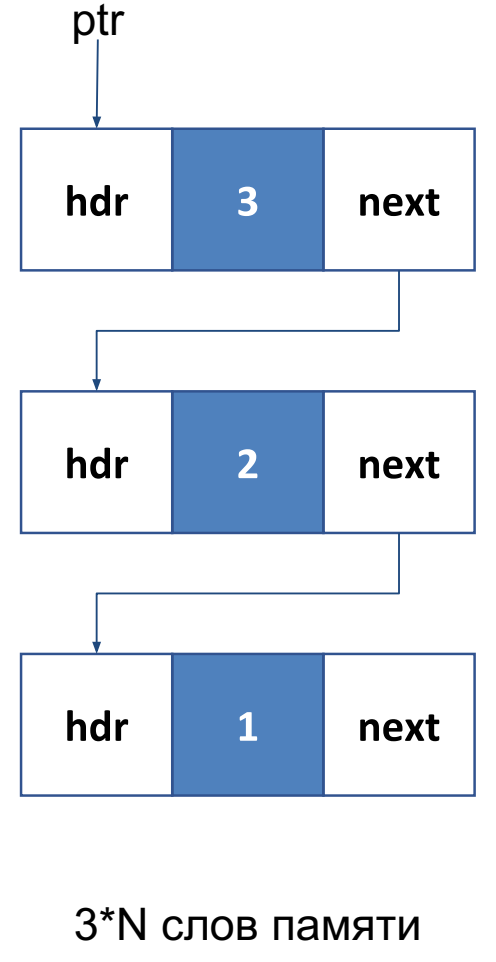
\includegraphics[width=0.2\linewidth]{pictures/List1}
	\caption{}
	\label{fig:list1}
\end{figure}

\begin{figure}[h!]
	\centering
	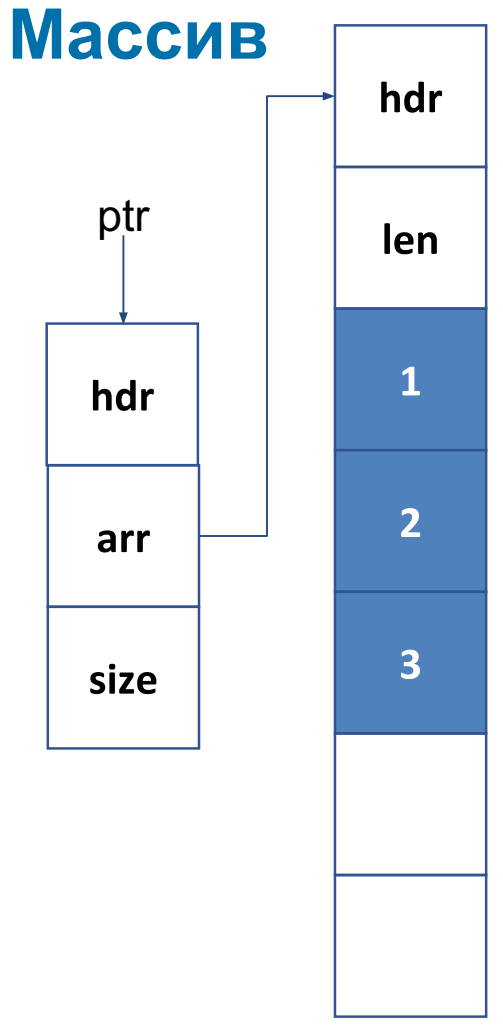
\includegraphics[width=0.1\linewidth]{pictures/Array1}
	\caption{}
	\label{fig:array1}
\end{figure}

\begin{figure}[h!]
	\centering
	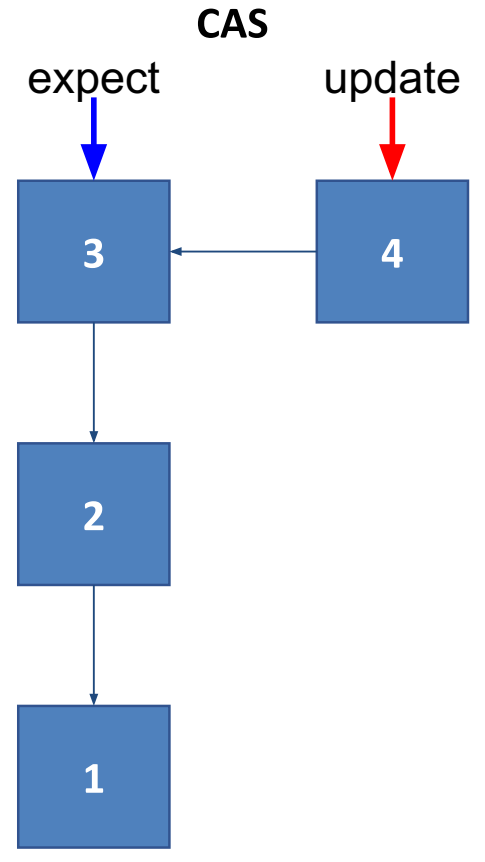
\includegraphics[width=0.2\linewidth]{pictures/List2}
	\caption{Стек на списке}
	\label{fig:list2}
\end{figure}

\begin{figure}[h!]
	\centering
	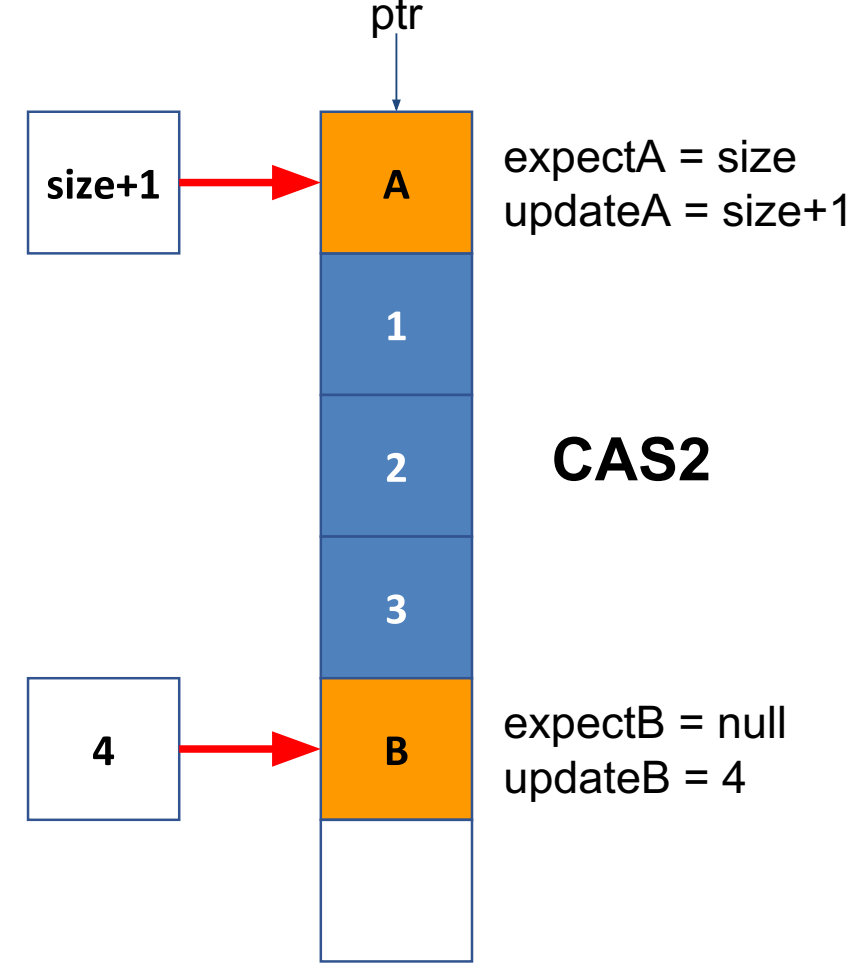
\includegraphics[width=0.4\linewidth]{pictures/Array2}
	\caption{Стек на массиве}
	\label{fig:array2}
\end{figure}


\subsection{CASn}

\begin{lstlisting}
class Ref<T>(intial: T) {
   var _v = atomic<Any?>(initial)
   
   var value: T
       get() {
          return _v as T //TODO
       }
       
       set(upd) {
           this._v = upd //TODO
       }
}
\end{lstlisting}

\subsubsection{DCSS}

\begin{enumerate}
	\item Рисунок \ref{fig:dcss1}
    \item Рисунок \ref{fig:dcss2}
    \item Рисунок \ref{fig:dcss3}
    \item Рисунок \ref{fig:dcss4}
    \item Рисунок \ref{fig:dcss5}
    \item Рисунок \ref{fig:dcss6}
\end{enumerate}

\begin{figure}[h!]
	\centering
	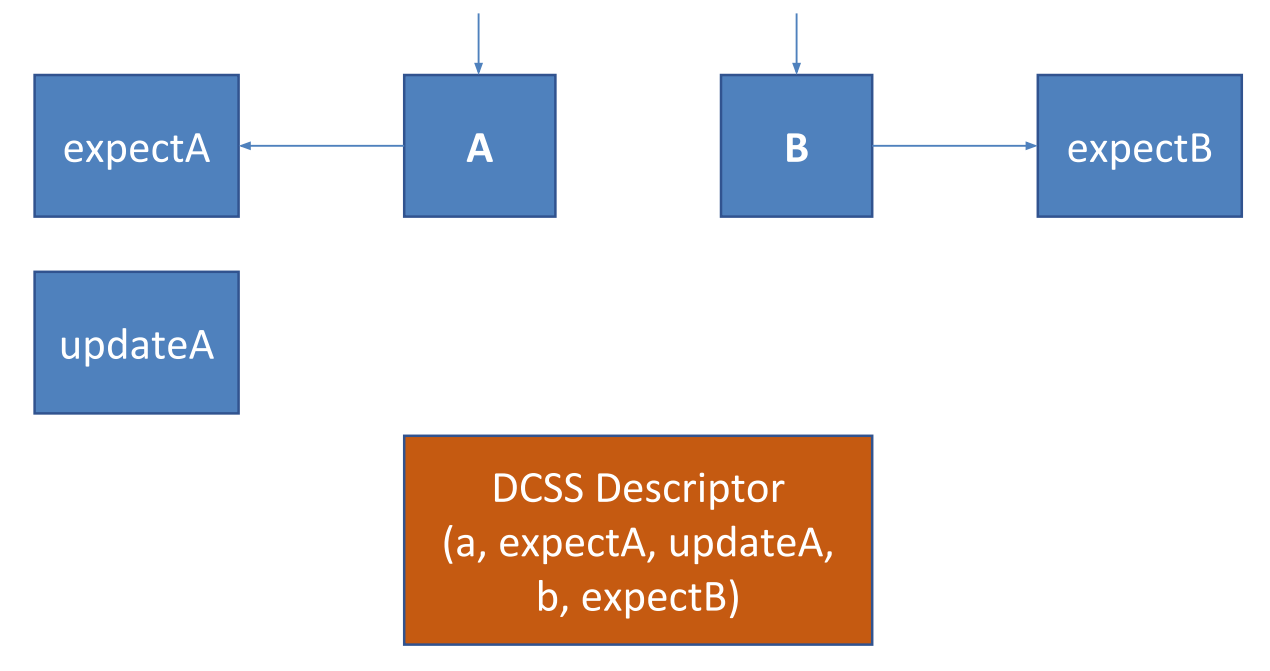
\includegraphics[width=0.4\linewidth]{pictures/DCSS1}
	\caption{init descriptor}
	\label{fig:dcss1}
\end{figure}

\begin{figure}[h!]
	\centering
	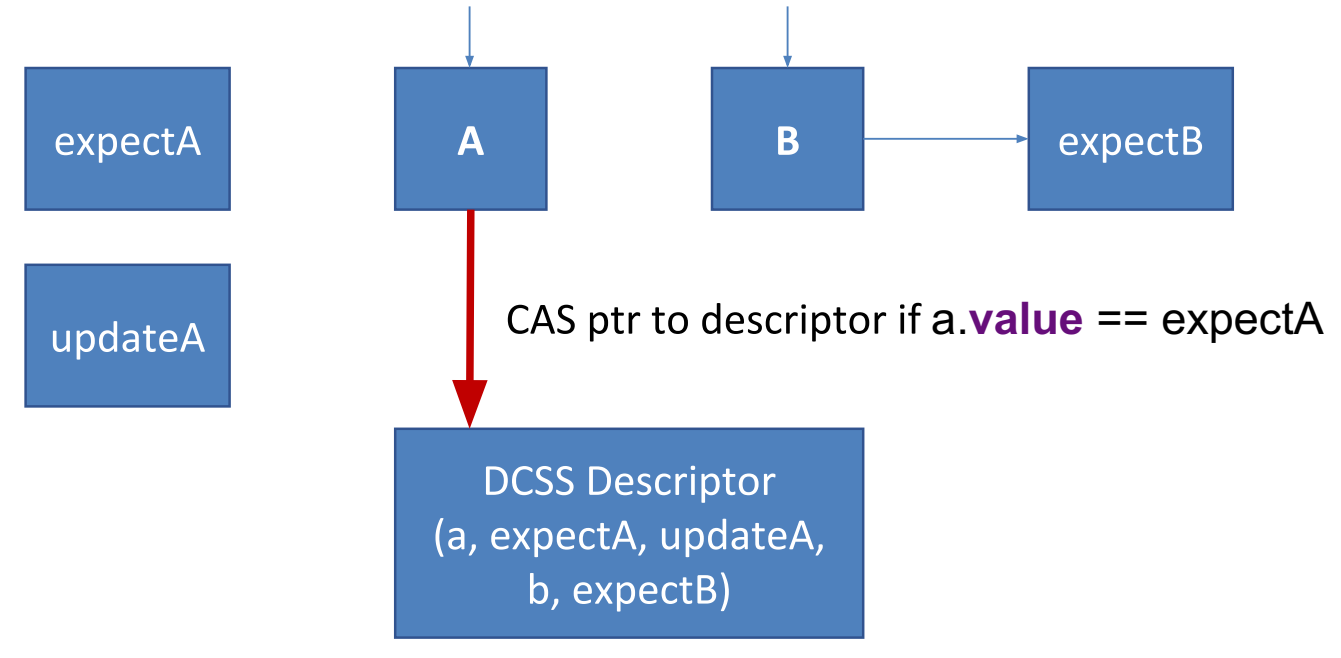
\includegraphics[width=0.4\linewidth]{pictures/DCSS2}
	\caption{prepare}
	\label{fig:dcss2}
\end{figure}

\begin{figure}[h!]
	\centering
	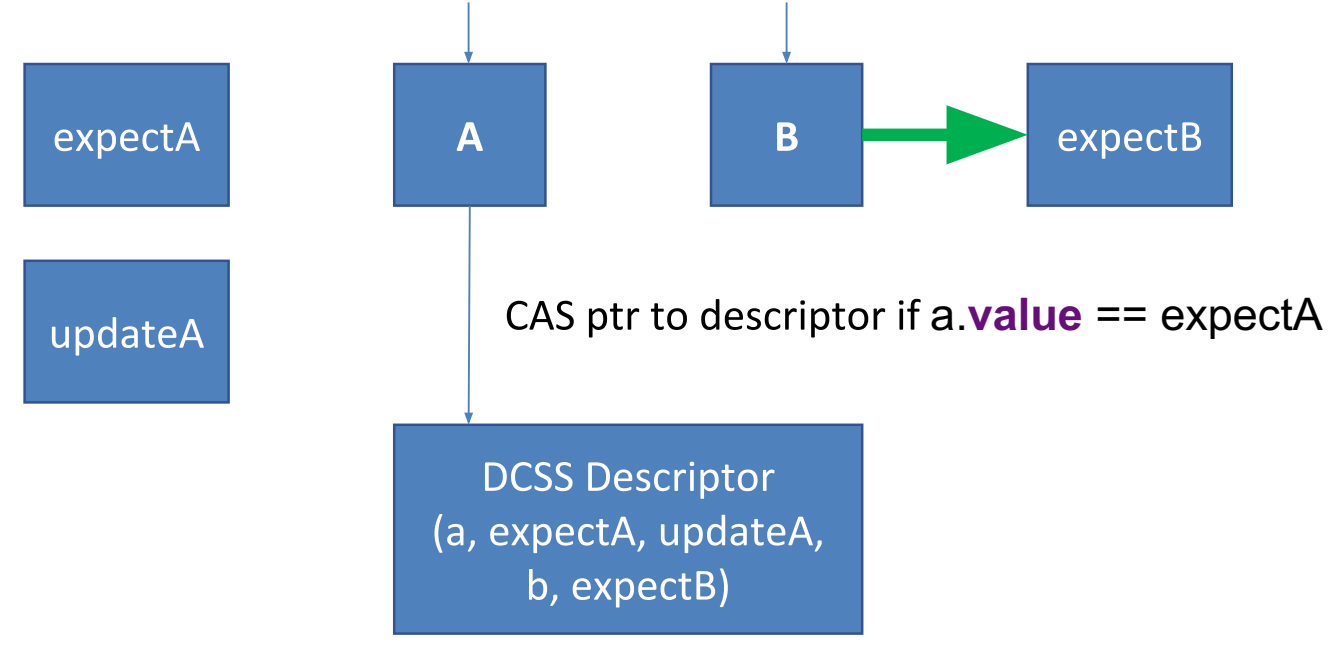
\includegraphics[width=0.4\linewidth]{pictures/DCSS3}
	\caption{read b.value}
	\label{fig:dcss3}
\end{figure}

\begin{figure}[h!]
	\centering
	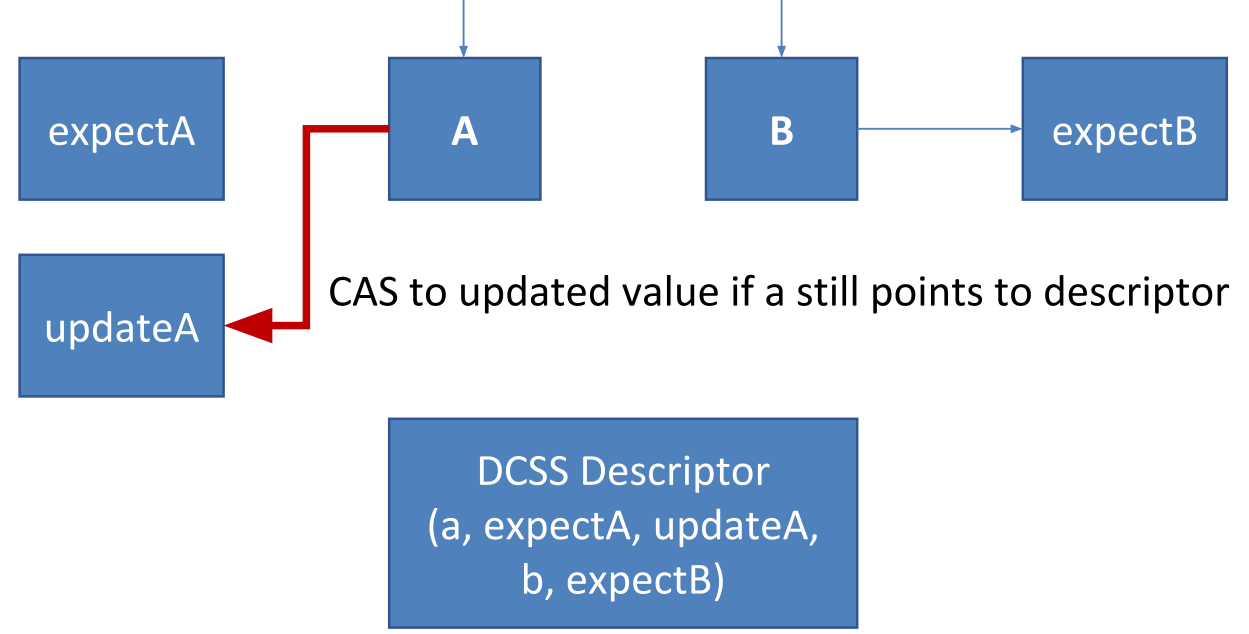
\includegraphics[width=0.4\linewidth]{pictures/DCSS4}
	\caption{complete when success}
	\label{fig:dcss4}
\end{figure}

\begin{figure}[h!]
	\centering
	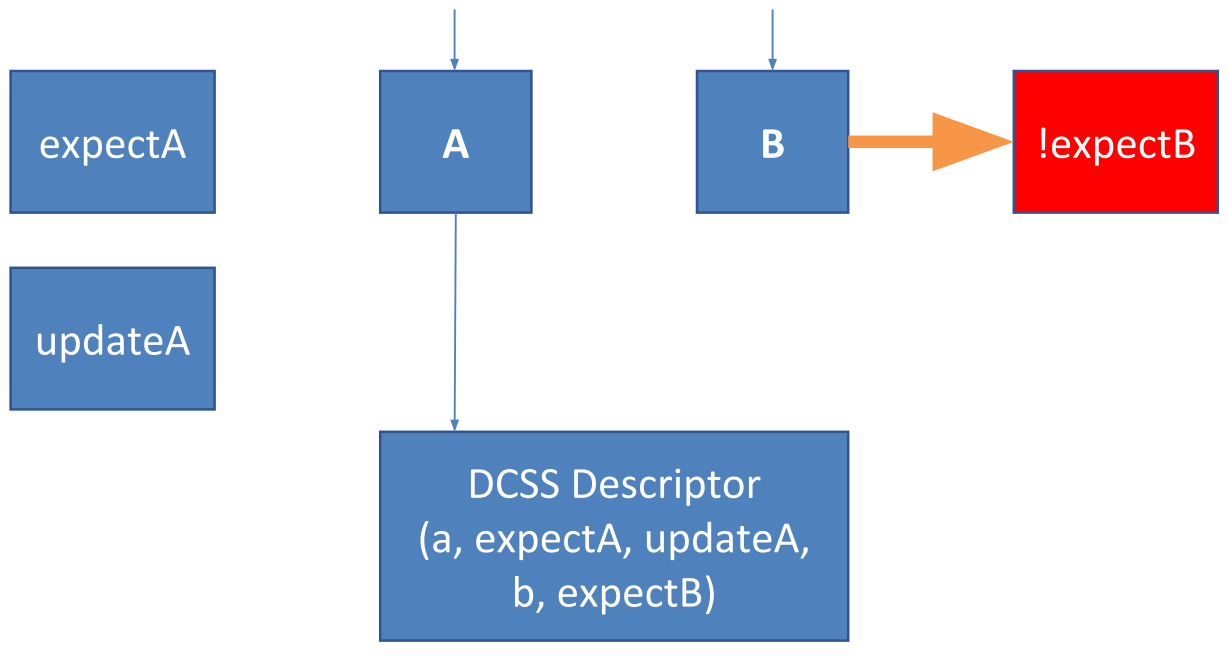
\includegraphics[width=0.4\linewidth]{pictures/DCSS5}
	\caption{complete (alternative)}
	\label{fig:dcss5}
\end{figure}

\begin{figure}[h!]
	\centering
	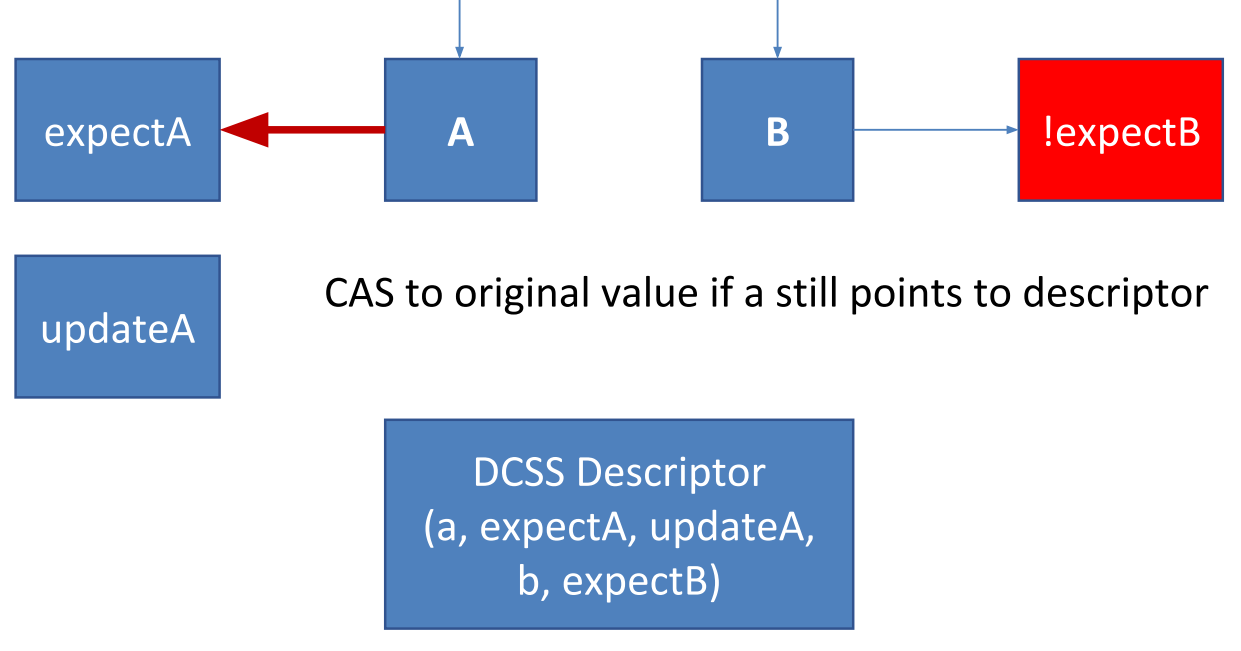
\includegraphics[width=0.4\linewidth]{pictures/DCSS6}
	\caption{compete when failed}
	\label{fig:dcss6}
\end{figure}

\begin{figure}[h!]
	\centering
	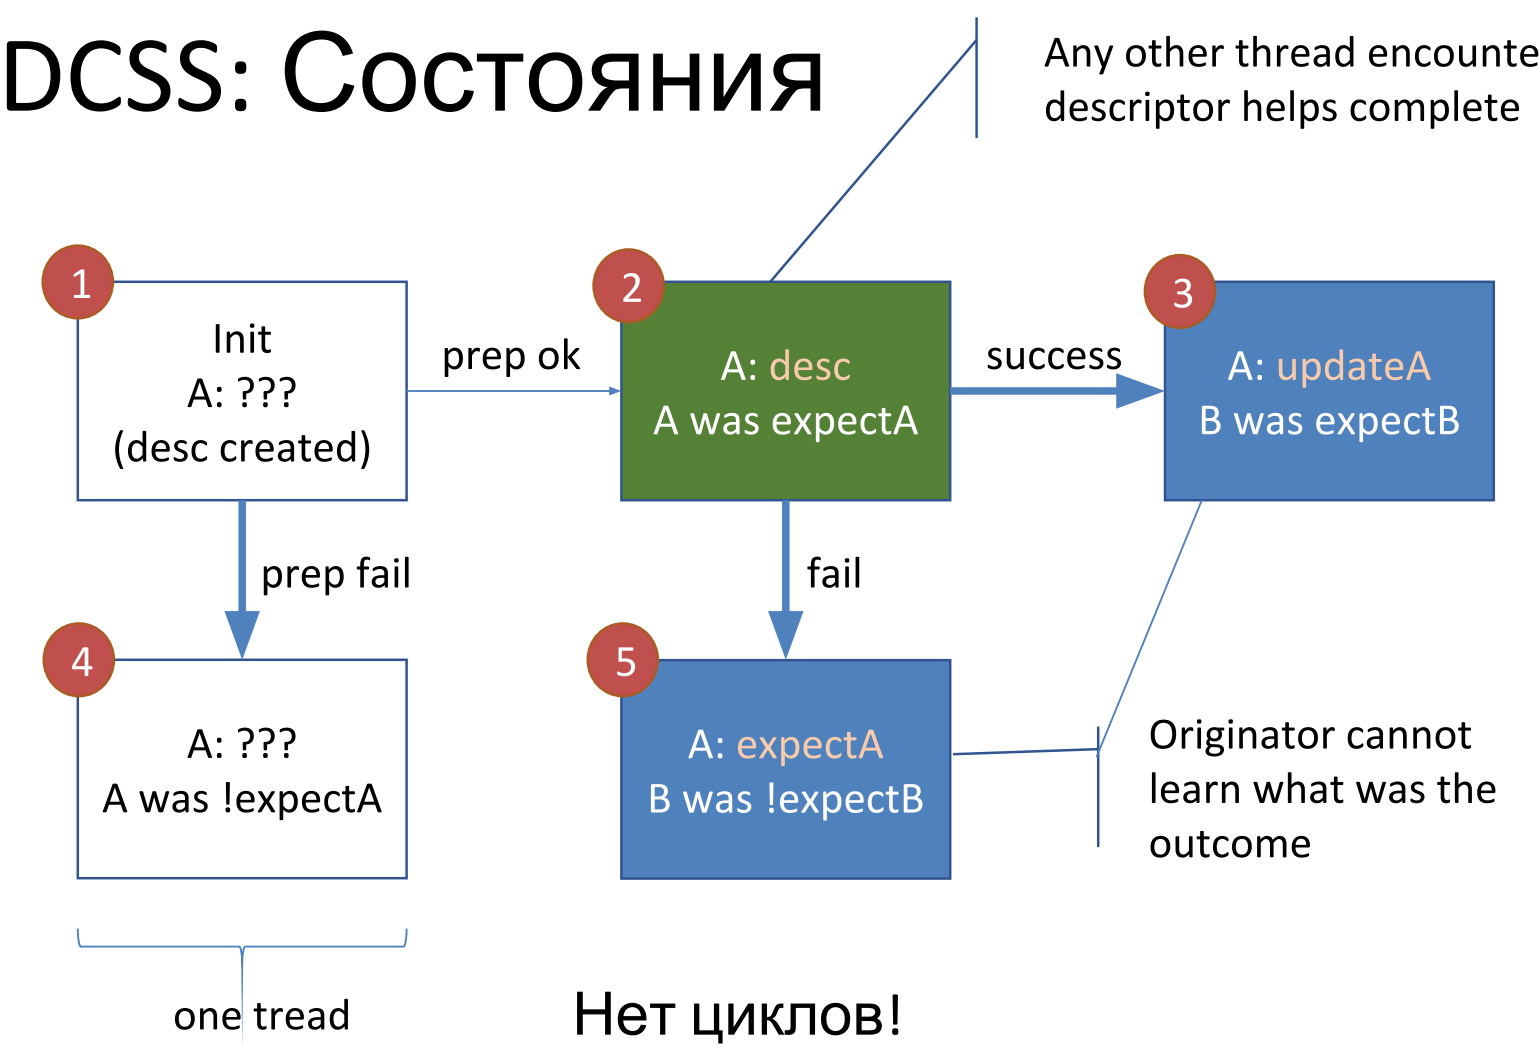
\includegraphics[width=0.5\linewidth]{pictures/DCSS7}
	\caption{DCSS all}
	\label{fig:dcss7}
\end{figure}

\paragraph{Псевдокод}

\begin{lstlisting}
fun <A,B> dcss(
    a: Ref<A>, expectA: A, updateA: A,
    b: Ref<B>, expectB: B) =
    atomic {
        if (a.value == expectA && b.value == expectB) {
            a.value = updateA
        }
    }
\end{lstlisting}

\subsection{Наблюдения и замечания}

\begin{itemize}
	\item complete работает без циклов
	\subitem Реализует state machine кторая идёт только вперёд
	\item Но есть циклы помощи другим потокам
	\subitem Алгоритм lock-free
	\item Адреса A \& B должны быть упорядочены
	\subitem Либо может переполниться стек при помощи
	\item Один из способов: Restricted DCSS (RDCSS)
	\subitem A и B берутся из разных "регионов" (не пересекающихся) 
\end{itemize}

\subsection{Подход к реализации}

\begin{lstlisting}
abstract class Descriptor {
    abstract fun complete()
}

class Ref<T>(initial: T) {
    var _v = atomic<Any?>(initial)
    
    var value: T
        get() {
            _v.loop{ cur -> 
                when(cur) {
                    is Descriptor -> cur.complete()
                    else -> return cur
                }
            }
        }
        
        set(upd) {
            _v.loop{ cur ->
                when(cur) {
                    is Descriptor -> cur.complete()
                    else -> if (_v.compareAndSet(cur, upd))
                        return
                }
            }
        }
}

class RDCSSDescriptor<A, B>(val a: Ref<A>, val expectA: A, val updateA: A, val b: Ref<B>, val expectB: B): Descriptor() {
    override fun complete() {
        val update = if (b.value == expectB) updateA else expectA
        a._v.compareAndSet(this, update)
    }
}
\end{lstlisting}

\subsection{DCSS Mod}

\begin{enumerate}
	\item Рисунок \ref{fig:dcssm1}
	\item Рисунок \ref{fig:dcssm2}
	\item Рисунок \ref{fig:dcssm3}
	\item Рисунок \ref{fig:dcssm4}
	\item Рисунок \ref{fig:dcssm5}
\end{enumerate}

\begin{figure}[h!]
	\centering
	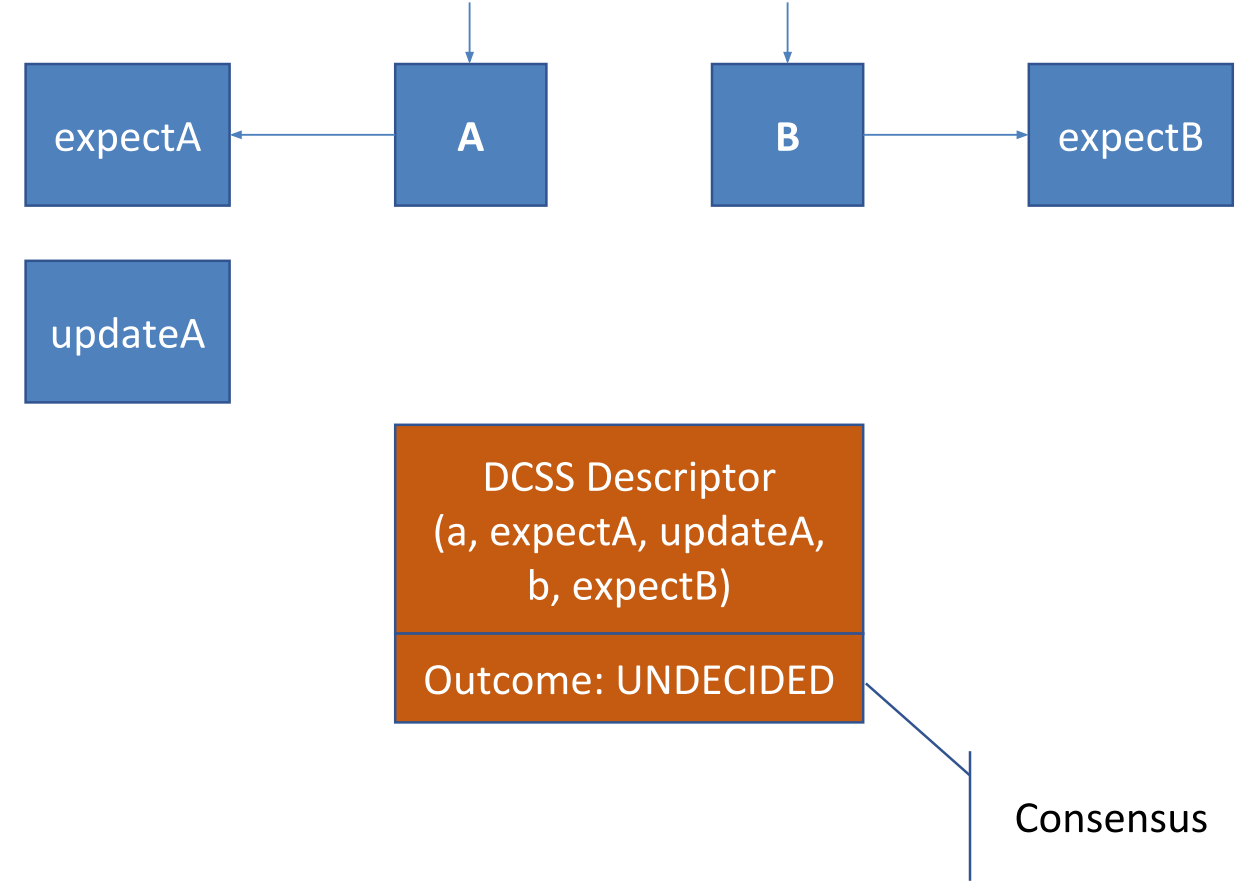
\includegraphics[width=0.4\linewidth]{pictures/DCSSM1}
	\caption{init state}
	\label{fig:dcssm1}
\end{figure}

\begin{figure}[h!]
	\centering
	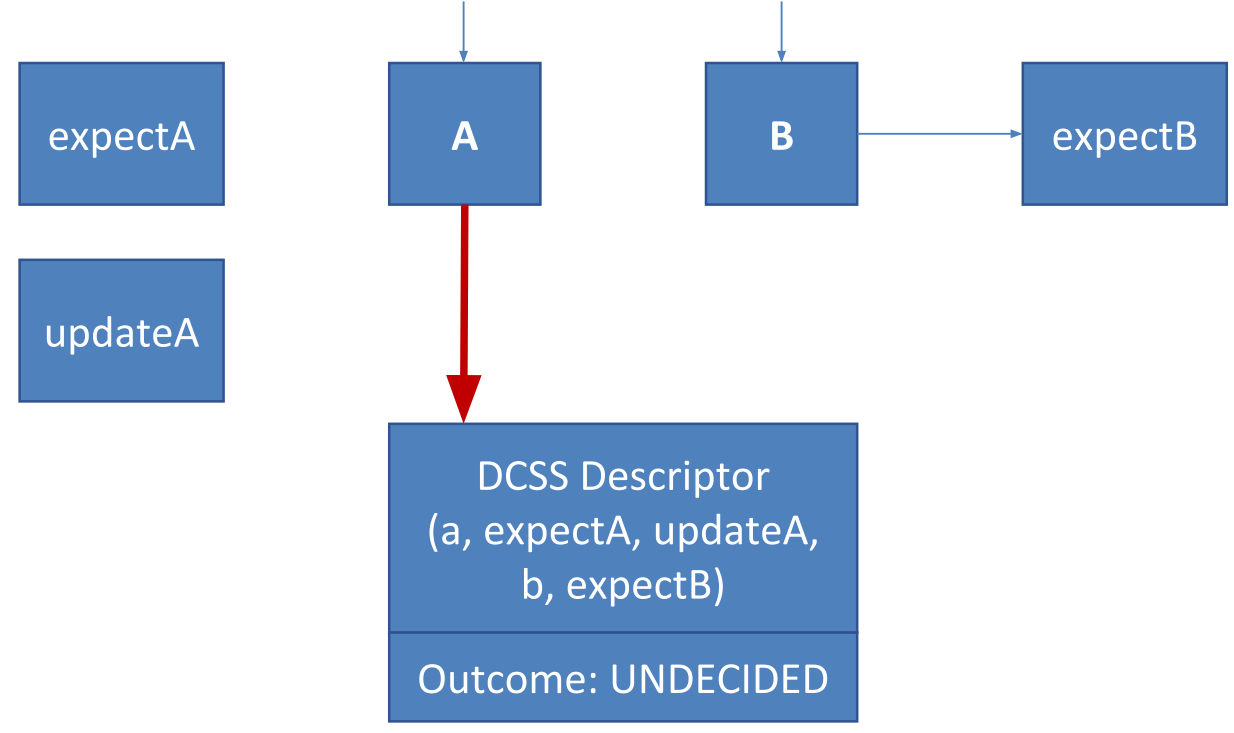
\includegraphics[width=0.4\linewidth]{pictures/DCSSM2}
	\caption{prepare}
	\label{fig:dcssm2}
\end{figure}

\begin{figure}[h!]
	\centering
	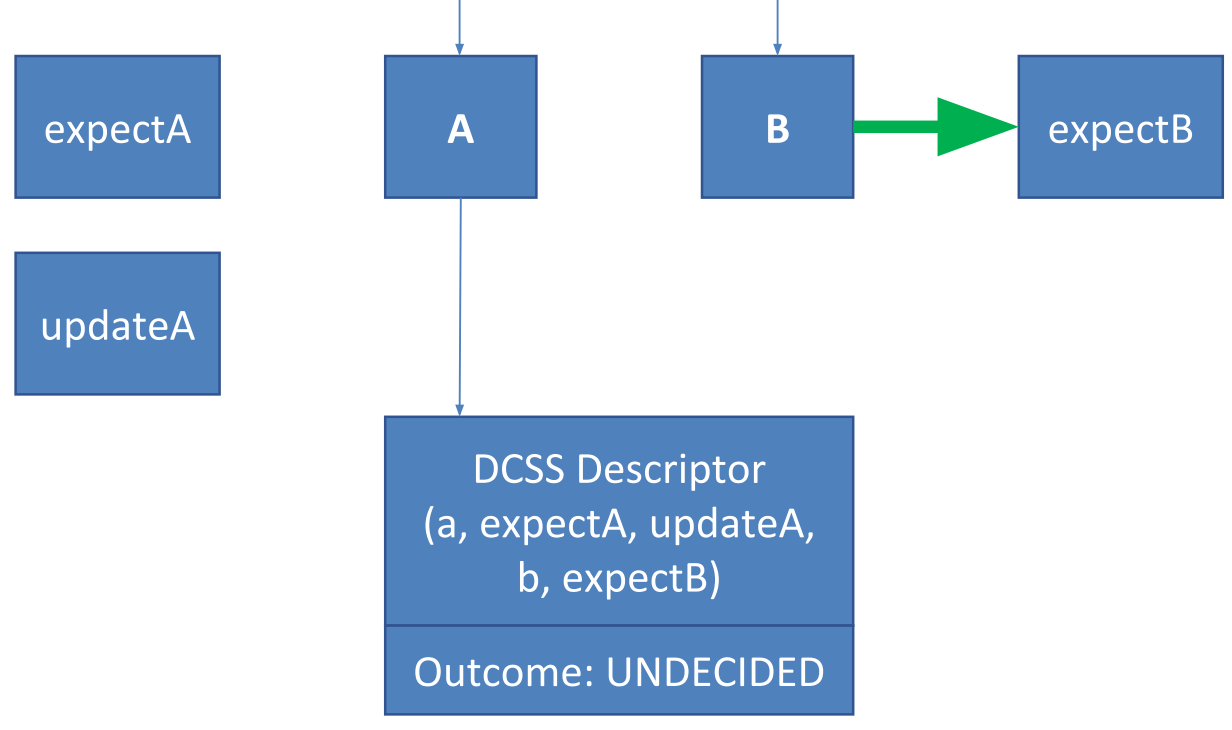
\includegraphics[width=0.4\linewidth]{pictures/DCSSM3}
	\caption{read b.value}
	\label{fig:dcssm3}
\end{figure}

\begin{figure}[h!]
	\centering
	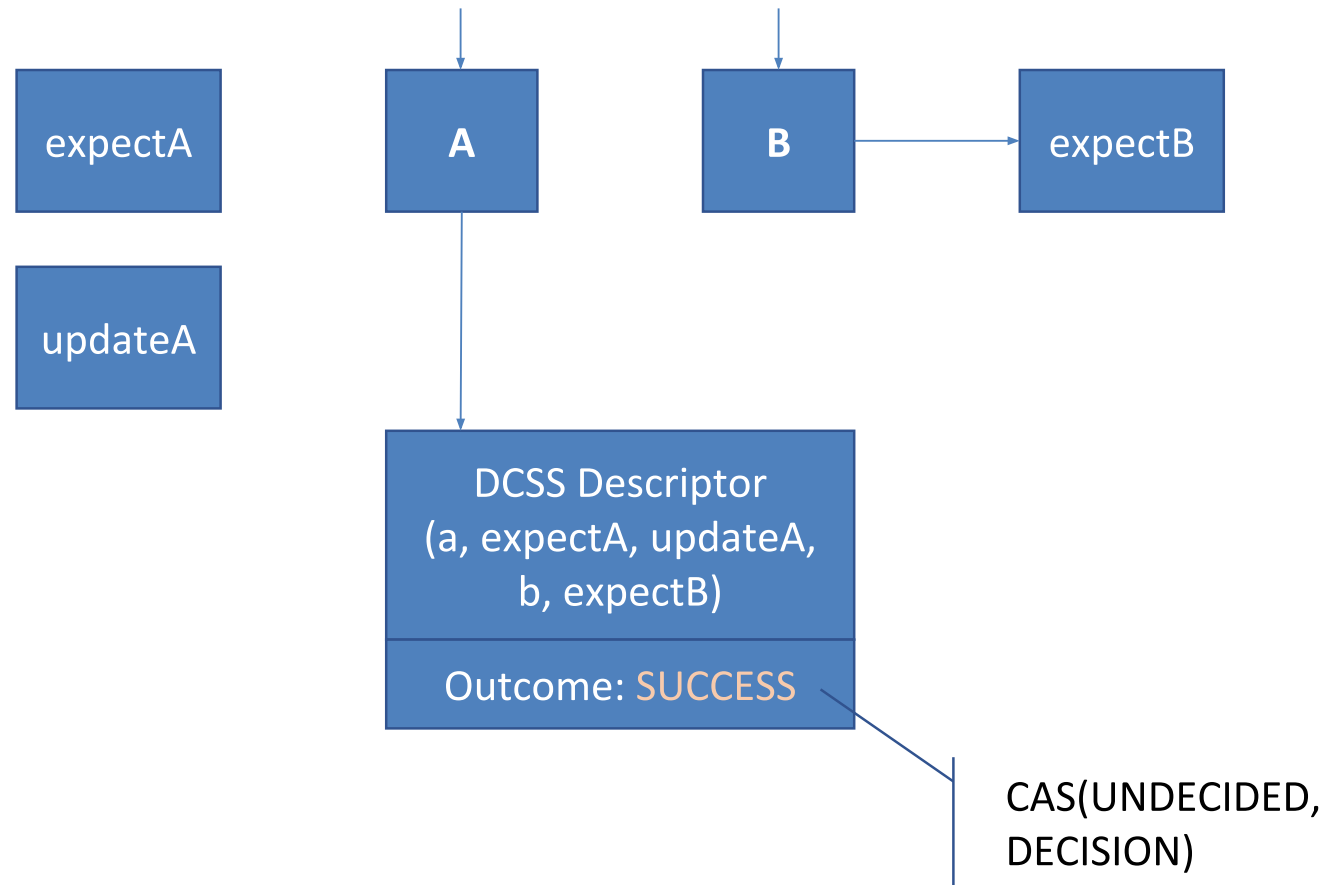
\includegraphics[width=0.4\linewidth]{pictures/DCSSM4}
	\caption{reach consensus}
	\label{fig:dcssm4}
\end{figure}

\begin{figure}[h!]
	\centering
	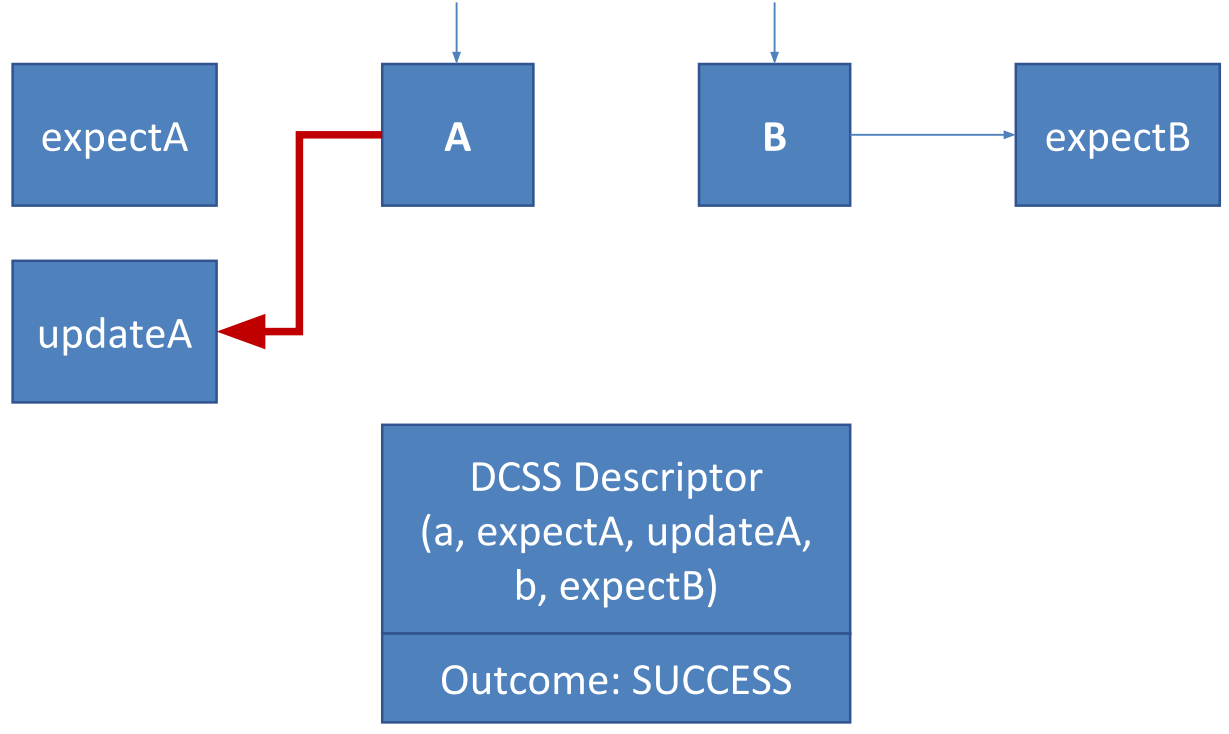
\includegraphics[width=0.4\linewidth]{pictures/DCSSM5}
	\caption{complete}
	\label{fig:dcssm5}
\end{figure}

\begin{figure}[h!]
	\centering
	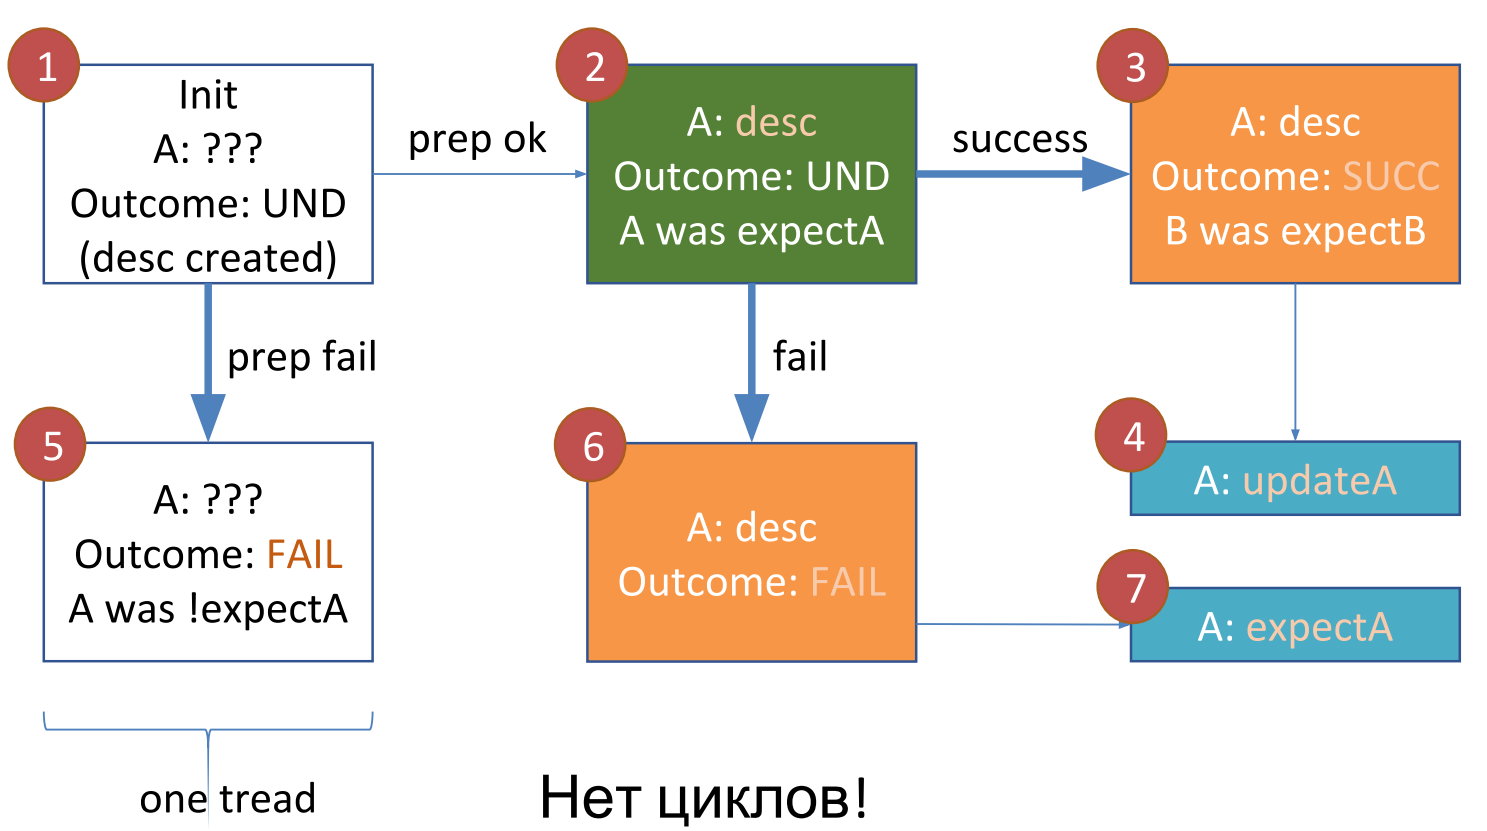
\includegraphics[width=0.5\linewidth]{pictures/DCSSM6}
	\caption{all states}
	\label{fig:dcssm6}
\end{figure}

\subsection{CASN}

\subsubsection{Псевдокод CAS2}

\begin{lstlisting}
fun <A,B> cas2(a: Ref<A>, expectA: A, updateA: A, b: Ref<B>, expectB: B, updateB: B): Boolean = atomic {
    if (a.value == expectA && b.value == expectB) {
        a.value = updateA
        b.value = updateB
        true
    } else {
        false
    }
}
\end{lstlisting}

\begin{enumerate}
	\item Рисунок \ref{fig:casn1}
	\item Рисунок \ref{fig:casn2}
	\item Рисунок \ref{fig:casn3}
	\item Рисунок \ref{fig:casn4}
	\item Рисунок \ref{fig:casn5}
	\item Рисунок \ref{fig:casn6}
\end{enumerate}

\begin{figure}[h!]
	\centering
	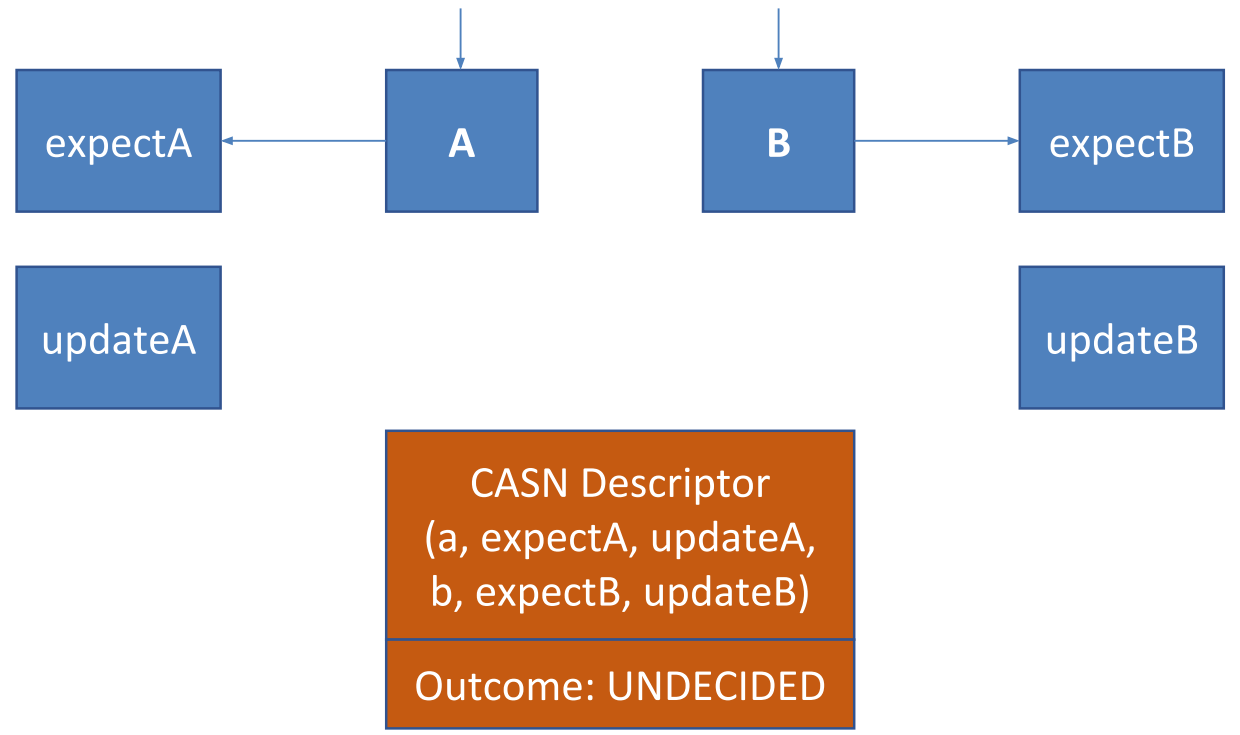
\includegraphics[width=0.4\linewidth]{pictures/CASN1}
	\caption{init descriptor}
	\label{fig:casn1}
\end{figure}

\begin{figure}[h!]
	\centering
	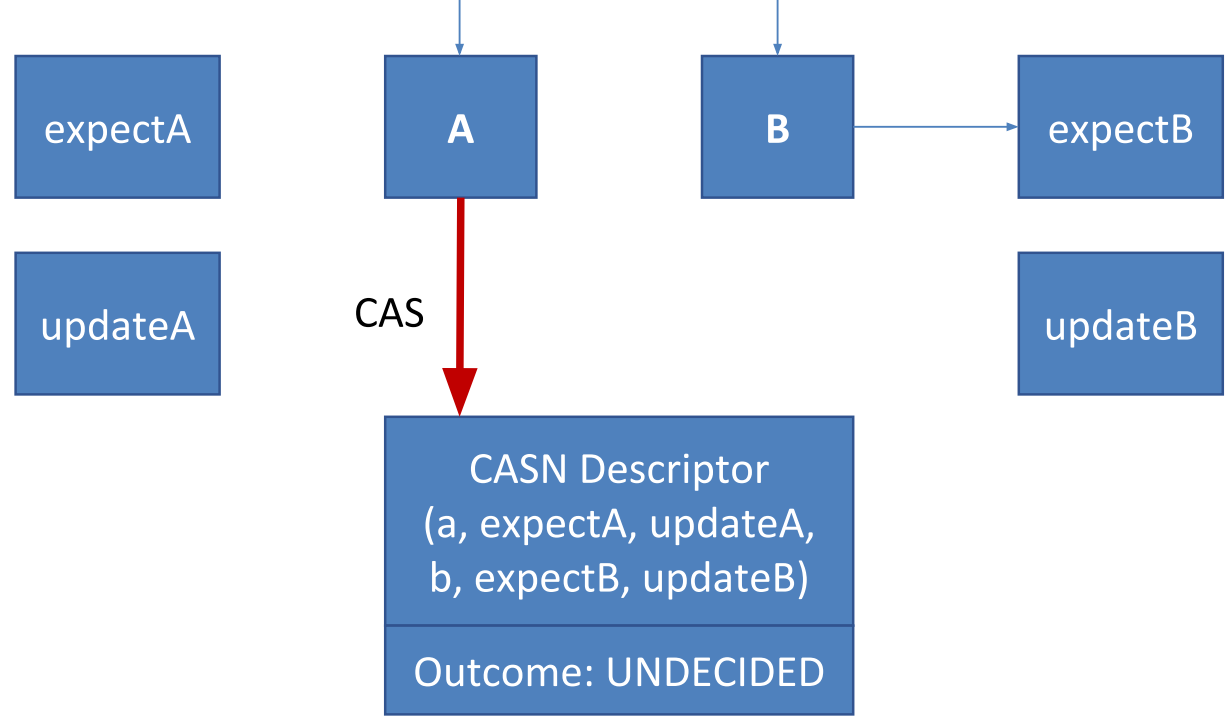
\includegraphics[width=0.4\linewidth]{pictures/CASN2}
	\caption{prepare(1)}
	\label{fig:casn2}
\end{figure}

\begin{figure}[h!]
	\centering
	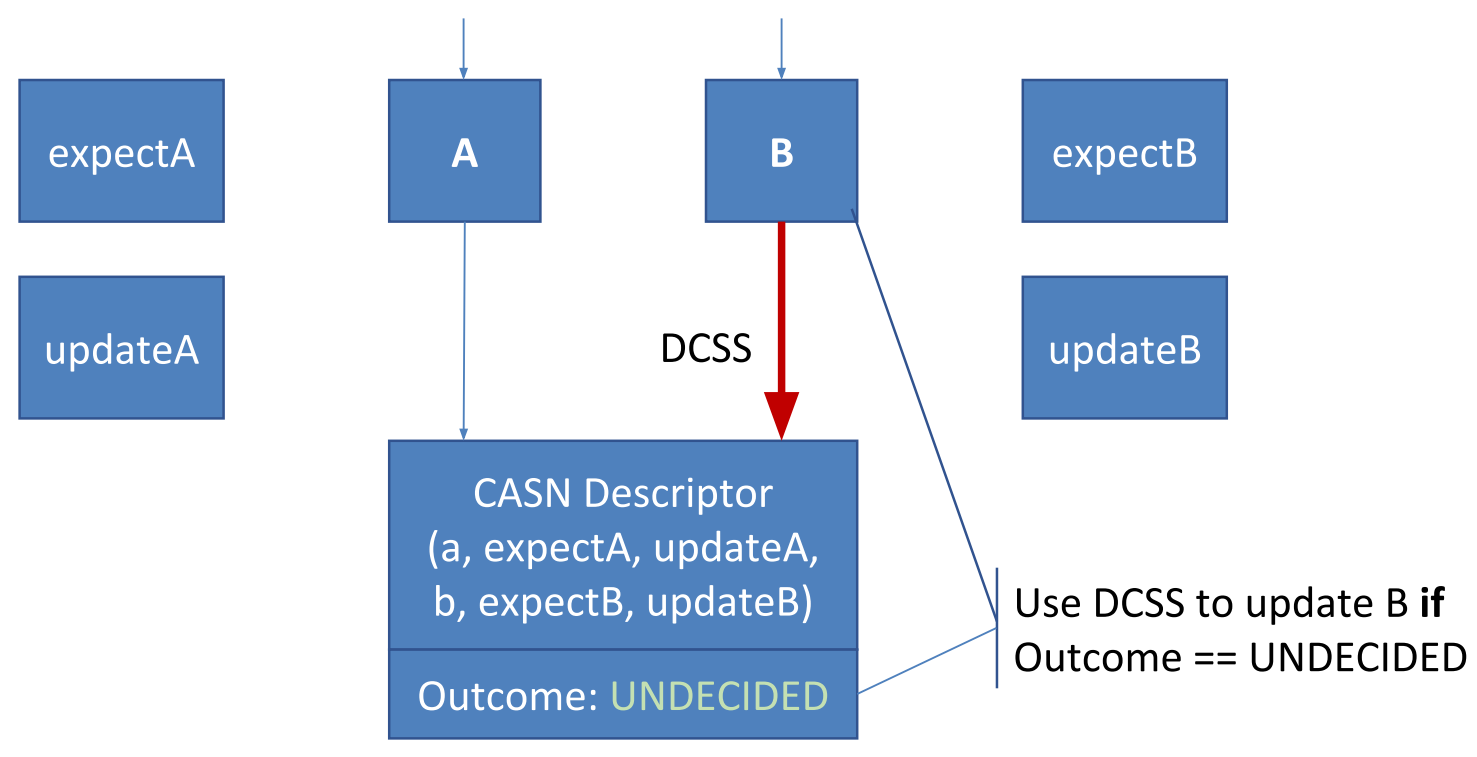
\includegraphics[width=0.4\linewidth]{pictures/CASN3}
	\caption{prepare(2)}
	\label{fig:casn3}
\end{figure}

\begin{figure}[h!]
	\centering
	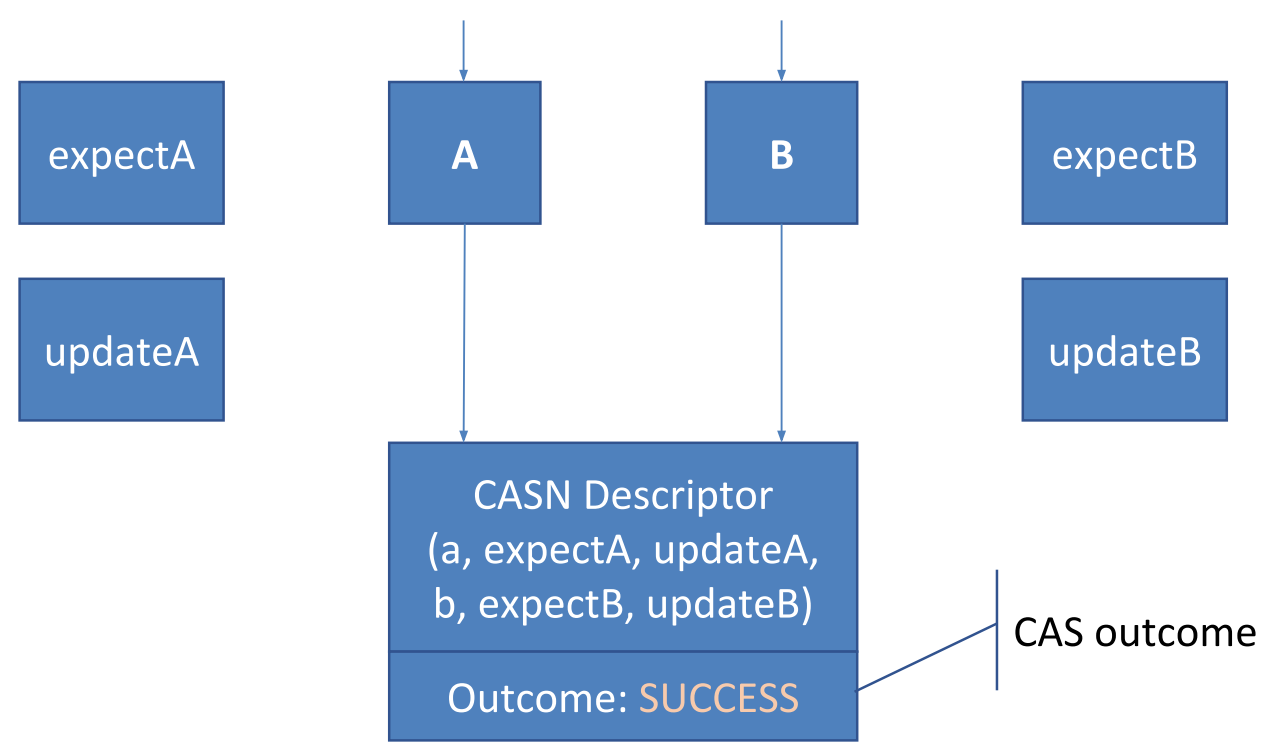
\includegraphics[width=0.4\linewidth]{pictures/CASN4}
	\caption{decide}
	\label{fig:casn4}
\end{figure}

\begin{figure}[h!]
	\centering
	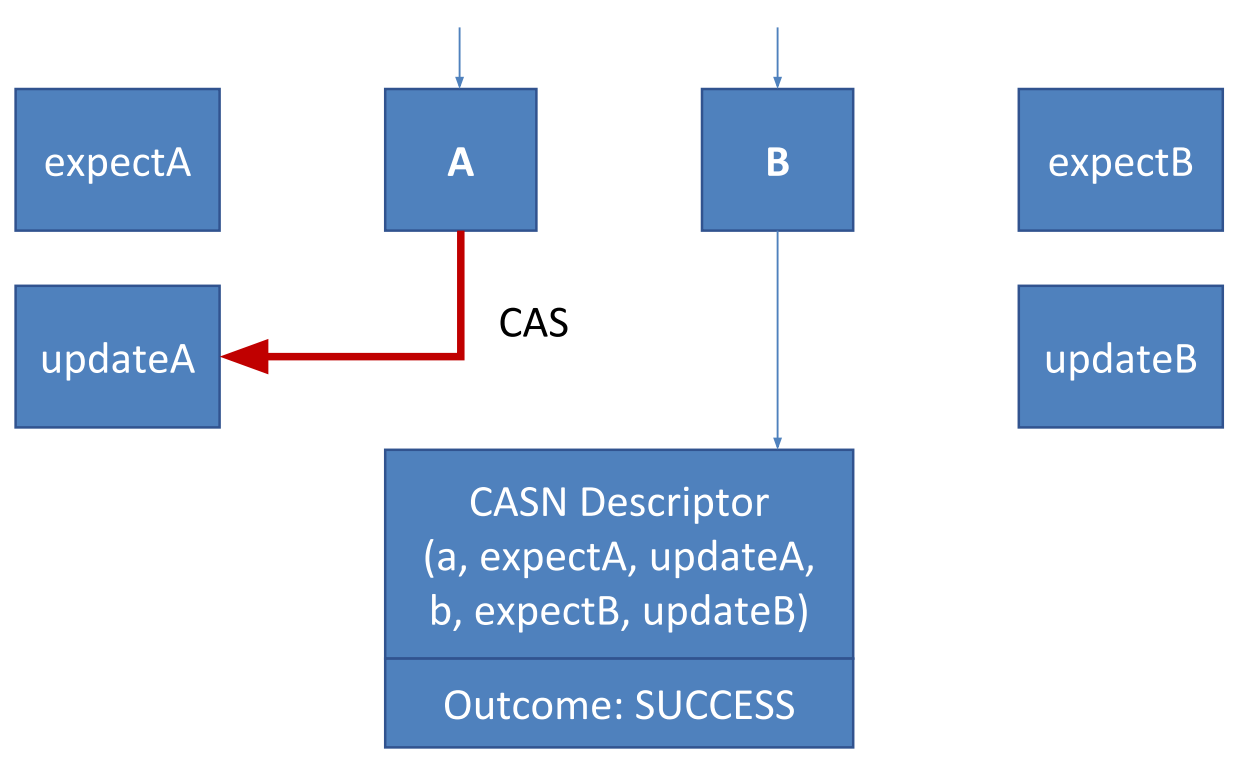
\includegraphics[width=0.4\linewidth]{pictures/CASN5}
	\caption{complete(1)}
	\label{fig:casn5}
\end{figure}

\begin{figure}[h!]
	\centering
	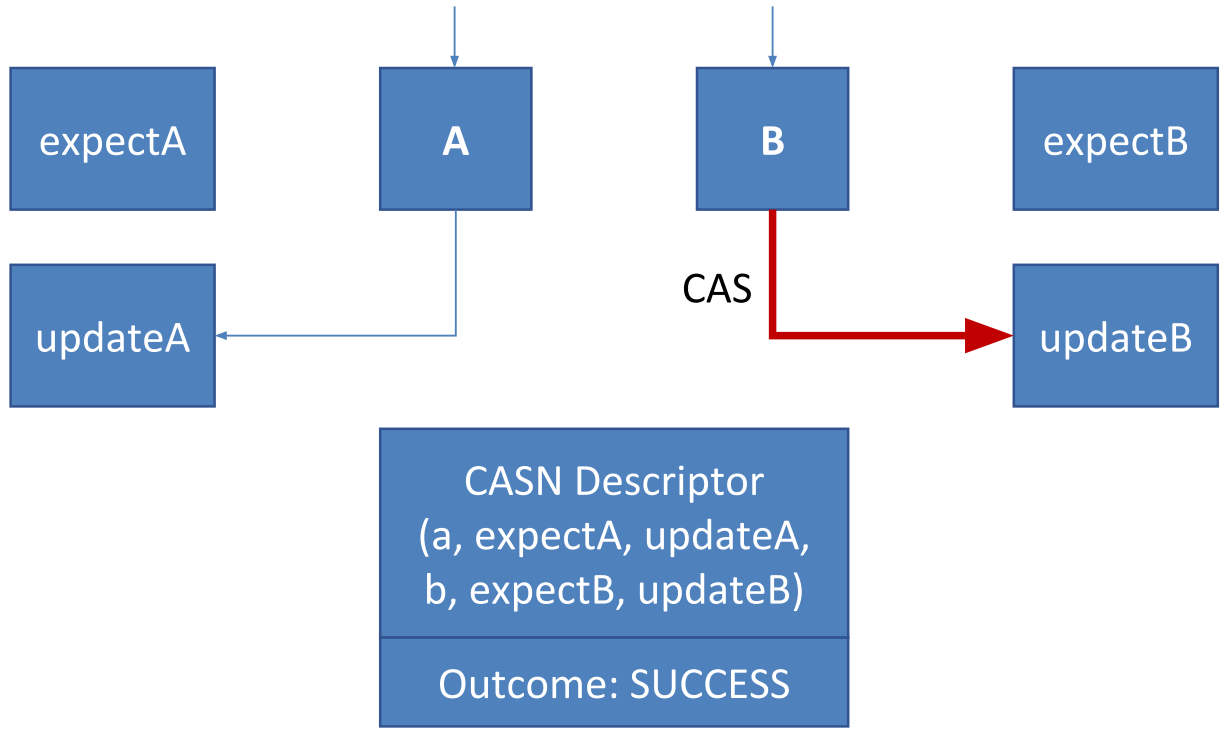
\includegraphics[width=0.4\linewidth]{pictures/CASN6}
	\caption{complete(2)}
	\label{fig:casn6}
\end{figure}

\begin{figure}[h!]
	\centering
	\includegraphics[width=0.5\linewidth]{pictures/CASN7}
	\caption{all states}
	\label{fig:casn7}
\end{figure}

\section{Мониторы и ожидание}

\subsection{Объекты как функции}
\begin{itemize}
	\item Операция над объектом как функция $f(S, P)=(S', R)$
	\item Ранее опеарции были {\bfseries всюду определены} на паре $(S, P)$
	\begin{itemize}
		\item Если операцию нельзя выполнить, то результат --- ошибка или исключение
	\end{itemize}
    \item В общем случае операции могут быть {\bfseries частично определены} на множестве пар $(S, P)$
    \begin{itemize}
    	\item Операция не может завершиться и \emph{ждёт}
    \end{itemize}
\end{itemize}

\subsection{Очередь ограниченного размера с ожиданием}

\begin{itemize}
	\item Обычные операции
	\begin{itemize}
		\item {\bfseries size(): int} --- узнать текущий размер
		\item {\bfseries offer(item): Boolean} --- вернет {\bfseries false} если свободнго места нет
		\item {\bfseries poll(): item?} --- вернёт {\bfseries null} если очередь пуста
	\end{itemize}
    \item Операции с ожиданием
    \begin{itemize}
    	\item {\bfseries put(item)} --- положить элемент в очередь если есть свободное место (иначе ждёт, в этом состоянии операция не определена)
    	\item {\bfseries take(): item} --- взять элемент из очереди если она не пуста (иначе ждёт)
    \end{itemize}
\end{itemize}

\subsection{Лианеризуемость операций с ожиданием}
\begin{itemize}
	\item Расширим понятие исполнения
	\begin{itemize}
		\item Есть событие вызова inv(A)
		\item Но не обязателен ответ resp(A)
		\begin{itemize}
			\item\begin{defenition}
				A это {\bfseries незавершенная} операция, если нет resp(A)
			\end{defenition}
		    \item \begin{defenition}
		    	inv(A) --- это {\bfseries незавершенный вызов}
		    \end{defenition}
		\end{itemize}
	\end{itemize}
    \item \begin{defenition}
    	Исполнение {\bfseries лианеризуемо}
    	\begin{itemize}
    		\item Если для незавершенных операций можно
    		\begin{itemize}
    			\item Либо добавить ответы
    			\item Либо выкинуть их из исполнения
    	    \end{itemize}
            \item Чтобы получилось допустимое последовательное исполнение: $inv(A_1)\to reps(A_1)\to inv(A_2)\to resp(A_2)\ldots$
    	\end{itemize}
    \end{defenition}
    Рисунки \ref{fig:queuewait1} и \ref{fig:queuewait2}
\end{itemize}

\begin{figure}[h]
	\centering
	\includegraphics[width=0.4\linewidth]{pictures/QueueWait1}
	\caption{Лианеризуемое исполнение}
	\label{fig:queuewait1}
\end{figure}

\begin{figure}[h]
	\centering
	\includegraphics[width=0.4\linewidth]{pictures/QueueWait2}
	\caption{Нелианеризуемое исполнение}
	\label{fig:queuewait2}
\end{figure}

\begin{figure}[h!]
	\centering
	\includegraphics[width=0.4\linewidth]{pictures/QueueWait3}
	\caption{}
	\label{fig:queuewait3}
\end{figure}

\begin{figure}[h!]
	\centering
	\includegraphics[width=0.4\linewidth]{pictures/QueueWait4}
	\caption{}
	\label{fig:queuewait4}
\end{figure}

\subsection{Реализация через монитор}
{\bfseries Monitor = mutex + conditional variables}
\begin{itemize}
	\item Взаимное исключение для защиты данных от одновременного изменения
	\item Условные переменные для ожидания
	\item Мониторы придуманы Энтони Хоар (1974) (поэтому они также называются "Hoare monitors")
\end{itemize}

\subsection{Монитор в Java}

\begin{itemize}
	\item В Java каждый объект имеет монитор с \emph{одной} условной переменной
	\begin{itemize}
		\item {\bfseries synchronized}
		\begin{itemize}
			\item {\bfseries monitorenter} (lock)
			\item {\bfseries monitorexit} (unlock)
		\end{itemize}
		\item {\bfseries wait, notify, notifyAll} --- для работы с условной переменной
	\end{itemize}
\end{itemize}

В некотрых сстемах wait() реализован как хэш-таблица, при чем при коллизии кого-нибудь разбудим Поэтому ждать нужно в цикле, чтобы каждый раз проверяь условие.

Wait() и notify() можно использовать только внутри критической секции (в synchronized)

Так как в мониторе только одна условная переменная, то, если у нас есть потоки ожидающие разных событий, то мы не можем использовать метод notify(), так как мы можем разбудить не тот поток и, поэтому тоже wait надо использовать в цикле.

\subsection{Циклическая очередь с ожиданием на массиве}

\begin{lstlisting}[language=Java]
public class BlockingQueue<T> {
    privite final T[] items;
    privite final int n;
    privite int head;
    privite int tail; 
}
\end{lstlisting}

\subsubsection{size()}

Испльзуем грубую синхронизацию через встроенный в Java объекты монитор

\begin{lstlisting}[language=Java]
privite synchronized int size() {
    return (tail - head + ) % n;
}
\end{lstlisting}

\subsubsection[poll()]{Неждущий poll()}

\begin{lstlisting}[language=Java]
public synchronized T poll() {
    if (head == tail) return null;
    T result = items[head];
    items[head] = null;
    if ((tail + 1) % n == head) notifyAll();
    head = (head + 1) % n;
    return result; 
}
\end{lstlisting}

\subsubsection[take()]{Ждущий take()}

\begin{lstlisting}[language=Java]
public synchronized T take() throws InterruptedException {
    while (head == tail) wait();
    T result = items[head];
    items[head] = null;
    if ((tail + 1) % n == head) notifyAll();
    head = (head + 1) % n;
    return result;
}
\end{lstlisting}

\subsubsection[offer()]{Неждущий offer()}

\begin{lstlisting}[language=Java]
public synchronized boolean offer(T item) {
    int next = (tail + 1) % n;
    if (next == head) return false;
    items[tail] = item;
    if (tail == head) notifyAll();
    tail = next;
    return true;
}
\end{lstlisting}

\subsubsection[put()]{Ждущий put()}

\begin{lstlisting}[language=Java]
public synchronized void put(T item) throws InterruptedException {
    while (true) {
        int next = (tail + 1) % n;
        if (next == head) {
            wait();
            continue;
        }
        items[tail] = item;
        if (tail == head) notifyAll();
        tail = next;
        return;
    }
}
\end{lstlisting}

\subsection{notify() vs notifyAll()}

Если бы для каждого условия была своя отдельная переменная, то можно использовать {\bfseries notify()}. 

\subsection{ReentrantLock}

\begin{itemize}
	\item В пакете java.util.concurrent есть интерфейс {\bfseries Lock}
	\begin{itemize}
		\item С методами {\bfseries lock, unlock, newCondition}
		\item И {\bfseries ReentrantLock} --- его реализация
		\item Интерфейс {\bfseries Condition} для условных переменных с методами {\bfseries await, signal, signalAll}
		\item Можем завести отдельную переменную для каждого условия
	\end{itemize}
\end{itemize}

\begin{lstlisting}[language=Java]
privite final Lock lock = new ReentrantLock();
privite final Condition notFull = lock.newCondition();
privite final Condition notEmpty = lock.newCondition();
\end{lstlisting}

Но даже в этом случае мы не можем бездумно использовать signal

\subsubsection{Проблематичный сценарий}

\begin{itemize}
	\item Рассмотрим такую последовательность операций (рисунок~\ref{fig:queuewait5})
	\begin{enumerate}
		\item Два {\bfseries put} ждут {\bfseries notFull}
		\item Пришёл {\bfseries take}, сделал очередь неполной, послал {\bfseries notFull}
		\item Но один из {\bfseries put} не успел проснуться и взять {\bfseries lock} по сигналу
		\item Пришёл ещё {\bfseries take}. Очередь уже не полная, так что он не посылает еще один сигнал {\bfseries notFull}
	\end{enumerate}
    \item Итого: один {\bfseries put} проснулся, а другой продолжает спать, хотя очередь уже не полна
    \item Вывод: в отличии от {\bfseries notifyAll/signalAll} оптимизировать вызовы {\bfseries notify/signal} нужно осторожно (в данном случае нельзя)
\end{itemize}

\begin{figure}[h!]
	\centering
	\includegraphics[width=0.4\linewidth]{pictures/QueueWait5}
	\caption{}
	\label{fig:queuewait5}
\end{figure}

\subsection{Подробней про interrupt}

\begin{itemize}
	\item У каждого потока есть \emph{interrupted} флаг
	\begin{itemize}
		\item Его ставит метод {\bfseries Thread.interrupt}
		\item Его проверяют методы {\bfseries wait, await} и тому подобное
		\item В случае обнаружения выставленного флага эти методы
		\begin{itemize}
			\item Прекращают ждать
			\item Сбрасывают флаг
			\item Кидают {\bfseries InterruptedException}
		\end{itemize}
	\end{itemize}
    \item Это {\bfseries кооперативный} способ прерывания заблокированных потоков
    \begin{itemize}
    	\item Не нужно знать что именно ждёт поток
    	\item Но не надейтесь, что это будет работать в случае использования сторонних библиотек 
    \end{itemize} 
\end{itemize}

\subsubsection{Ненужный InterruptedException}

Если нужно реализовать метод, который ждёт но не выкидывает {\bfseries InterruptedException}, то interrupted флаг надо перевыставить

\begin{lstlisting}[language=Java]
public T takeOrNull() {
    try {
        return take();
    } catch (InterruptedException e) {
        Thread.currentThread().interrupt();
        return null;
    }
}
\end{lstlisting} 

\subsection{Поток обрабатывающий очередь}

\begin{itemize}
	\item Заводим свой флаг сигнализирующий, что поток надо остановить
	\begin{itemize}
		\item В отличие от флага interrupted нет риска, что какой-то сторонний метод его случайно сбросит
	\end{itemize}
    \item Метод {\bfseries run} выходит в случае прерывания
    \begin{itemize}
    	\item Флаг interrupted перевыставлять не надо
    \end{itemize}
\end{itemize}

\begin{lstlisting}[language=Java]
public class DoSomething<T> extends Thread {
    privite final BlockingQueue<T> queue;
    privite volatile boolean closed;
    
    public void close() {
        close = true;
        interrupt();
    }
    
    @Override
    public void run() {
        try {
            while(!closed) {
                T item = queue.take();
                doSomething(item);
            }
        } catch (InterruptedException e) {
            //ignore exception
        }
    }
}
\end{lstlisting}

\subsection{Ожидание без блокировки}

{\bfseries Пример: обновляемое значение}
\begin{itemize}
	\item Почти очередь на один элемент
	\item Операции
	\begin{itemize}
		\item {\bfseries update(item)} --- обновить текущее значение
		\item {\bfseries remove():item?} --- забрать и сбросить текущее значение
		\item {\bfseries take():item} --- ждёт пока новое значение появится
	\end{itemize}
\end{itemize}

\subsubsection{Реализация с блокиовкой}

\begin{lstlisting}
class DataHolder<T> {
    privite var value: T? = null
    privite val lock = ReentrantLock()
    privite val updated = lock.newCondition()
    
    fun update(item: T) = lock.withLock {
        value = item
        updated.signal()
    }
    
    fun remove(): T? = lock.withLock {
        value.also {value = null}
    }
    
    fun take(): T = lock.withLock {
        while (value == null) updated.await()
        value!!.also {value = null}
    }
}
\end{lstlisting}

\subsubsection{Реализация без блокировок}

\begin{lstlisting}
class DataHolder<T> {
    privite val v = atomic<T?>(null)
    
    fun update(item: T) {
        v.value = item //volotile write
        LockSupprort.unpark()
    }
    
    fun remove(): T? {
       v.loop { cur -> 
           if (cur == null) return null
           if (v.compareAndSet(cur, null)) return cur
       }
    }
}
\end{lstlisting}

\paragraph{Ожидание без блокировки (park())}

Здесь важен порядок: обновить $\to$ разбудить ({\bfseries unpark()})

\begin{lstlisting}
class TakerThread<T>: Thread() {
    //...
    
    fun take(): T {
        assert (Thread.currentThread() == this) 
        v.loop { cur -> 
            if (cur == null) {
                LockSupport.park()
                if (interrupted()) {
                    throw InterruptedException()
                }
                return@loop //continue
            }
            if (c.vompareAndSet(cur, null)) return cur
        }
    }
}
\end{lstlisting}

\begin{figure}[h!]
	\centering
	\includegraphics[width=0.5\linewidth]{pictures/Park}
	\caption{Магия park/unpark}
	\label{fig:park}
\end{figure}

\subsection{Ожидание из многих потоков}

\begin{itemize}
	\item Нужна очередь ждущих потоков
	\begin{itemize}
		\item Нетривиально написать
	\end{itemize}
    \item Возьмём готовую
    \item {\bfseries java.util.concurrent.lock.AbstractQueuedSynchronizer (рисунки \ref{fig:abstractqueuedsynchronizer1} и \ref{fig:abstractqueuedsynchronizer2})
    \begin{itemize}
    	\item ReentrantLock
    	\item ReentrantReadWriteLock
    	\item Semaphore
    	\item CountDownLatch
    \end{itemize}
}
\end{itemize}

\begin{figure}[h!]
	\centering
	\includegraphics[width=0.5\linewidth]{pictures/AbstractQueuedSynchronizer1}
	\caption{Анатомия AbstractQueuedSynchronizer(1)}
	\label{fig:abstractqueuedsynchronizer1}
\end{figure}

\begin{figure}[h!]
	\centering
	\includegraphics[width=0.5\linewidth]{pictures/AbstractQueuedSynchronizer2}
	\caption{Анатомия AbstractQueuedSynchronizer(2)}
	\label{fig:abstractqueuedsynchronizer2}
\end{figure}

\subsubsection{Пишем свой внутренний синхронайзер}

\begin{lstlisting}
inner class Sync: AbstractSynchronizer() {
    override fun tryAcquire(arg: Int): Boolean {
        val cur = v.value ?: return false
        if (!v.compareAndSet(cur, null)) return false
        //need to return value there
        results[arg] = cur
        return true
    }
    
    //always "release" --- wake up next thread
    override fun tryRelease(arg: Int): Boolean = true
}
\end{lstlisting}

\subsubsection{Используем его}

\begin{lstlisting}
privite val sync = Sync()

fun update(item: T) {
    v.value = item
    sync.release(0) //send signal
}

fun take(): T {
    val arg = reserveResultSlot()
    sync.acquireInterruptibly(arg) //wait inner
    //recheck for not lost unpark
    if (v.value != null) sync.release(0)
    return releaseResultSlot(arg)
}
\end{lstlisting}

\subsubsection{Улучшаем производительность}

\begin{itemize}
	\item Идея будить поток только когда обновляем: {\bfseries null} $\to$ значение
	\item Не работает очень тонким образом (рисунок~\ref{fig:fail})
	\subitem Из-за {\bfseries update} параллельный {\bfseries tryAcquire} может обламаться на CAS и запарковаться, но так как мы больше не вызываем {\bfseries release}, то никто его больше не разбудит
\end{itemize}

\begin{lstlisting}
fun update(item: T) {
    T old = v.getAndSet(item)
    if (old == null) sync.release(0)
}
\end{lstlisting}

\begin{figure}[h!]
	\centering
	\includegraphics[width=0.4\linewidth]{pictures/Fail}
	\caption{Fail}
	\label{fig:fail}
\end{figure}

\paragraph{Исправляем tryAcquire}

Используем цикл и повторяем, если CAS упал

\begin{lstlisting}
override fun tryAcquire(arg: Int): Boolean {
    while(true) {
        val cur = v.value ?: return false
        if (!v.compareAndSet(cur, null)) continue
        results[arg] = cur
        return true
    }
}
\end{lstlisting}

\section{FAA Based Queue}

\subsection{Fetch-And-Add}

\begin{itemize}
	\item FAA(adress, delta) --- атомарно увеличивает значение на delta и возвращает старое значение
	\item FAA гораздо лучше масштабируется, чем CAS
	\item Modern queues use Fetch-And-Add
\end{itemize}

\subsection{Obstruction-free queue on ifinite array}

\begin{itemize}
	\item Бескнечный массив и указатели для enqueue и dequeue. Сначала увеличиваем индекс потом пишем читаем.
	\item Если dequeue придёт читать раньше чем произошла запись, то мы пометим ячейку как сломанную и обе операции начнутся заново
\end{itemize}

\begin{lstlisting}
fun enqueue(x: T) = while(true) {
    val enqIdx = FAA(&this.enqIdx, 1)
    if (CAS(&data[enqIdx], null, x))
        return
}

fun dequeu(): T = while(true) {
    if (isEmpty()) return null
    val deqIdx = FAA(&this.deqIdx, 1)
    val res = SWAP(&data[deqIdx], BROKEN)
    if (res == null) continue
    else return (T) res
}

fun isEmpty(): Boolean = deqIdx >= neqIdx
\end{lstlisting}

\subsubsection{Michael-Scott queue of array segments}

\begin{figure}[h!]
	\centering
	\includegraphics[width=0.4\linewidth]{pictures/MSQueue1}
	\caption{MS queue of array segments}
	\label{fig:msqueue1}
\end{figure}

\begin{lstlisting}
fun enqueue(x: T) = while (true) {
    val tail = this.tail
    val enqIdx = FAA(&tail.enqIdx, 1)
    if (enqIdx >= NODE_SIZE) {
        //try to insert new Node with "x"
    } else {
        if (CAS(&data[enqIdx], null, x))
            return
    }
}

fun dequeue(): T = while(true) {
    val head = this.head
    if (head.isEmpty()) {
        val headNext = head.next ?: return null
        CAS(&this.head, head, headNext)
    } else {
        val deqIdx = FAA(&head.deqIdx, 1)
        if (deqIdx >= NODE_SIZE) continue
        val res = SWAP(&data[deqIdx], BROKEN)
        if (res == null) continue
        else return res
    }
}
\end{lstlisting}

\section{Counter Sharding}

\subsection{Naive counter}

\begin{lstlisting}
var counter = 0
fun inc() { FAA(&counter, 1)}
fun get():Int = counter
\end{lstlisting}

\begin{itemize}
	\item FAA берёт блокировку на уровне железа
	\item Часто вызываем inc $\Rightarrow$ contention на поле {\bfseries counter}
\end{itemize}

\subsection{Sharding}

\begin{itemize}
	\item get() вызывается сильно реже inc()
	\begin{itemize}
		\item Например, собирается какая-то perfomance метрика
	\end{itemize}
    \item Разобьём на несколько мини счётчиков (рисунок~\ref{fig:countersharding})
    \begin{itemize}
    	\item {\bfseries inc()} --- увеличивает случайный из них
    	\item {\bfseries get()} --- суммирует начения всех мини счётчиков
    \end{itemize}
\end{itemize}

\begin{figure}[h!]
	\centering
	\includegraphics[width=0.4\linewidth]{pictures/CounterSharding}
	\caption{Counter Sharding}
	\label{fig:countersharding}
\end{figure}



\section{Железо и спин-локи}
Так как у каждого ядра есть кэш, то он читает значение не и глобальной памяти, а из кэша, что ломает нам многопоточность. Решение - протокол MESI

\subsection{Backoff}
delay() - рандомизированный, т.к. если если несколько потоков ломанулись в блокировку и одному повезло, то он иожет очень быстро выполнить операцию и без делэя все остальные потоки снова ломанутся, это будет плохо, а если будет рандомищированный делэй, то кому-то из потоков повезет и он будет маленькое количество времени спать, и быстро схватит блокировку. Это очень важно, если у нас короткая блокировка.

Но этот алгоритм был нечестным, так как поток мог прийти последним и получить блокировку первым.

Напишем алгоритм с fist-come-first-served : CLH Lock

Isolation - пока транзакция работает, дригие не должны видеть несогласованный результат
Consistency - струдники не исчезают

\end{document}